% aliveKat
\documentclass[aps,pra,superscriptaddress,reprint,nofootinbib]{revtex4-1}
% \documentclass[prb,reprint,nofootinbib]{revtex4-1} 
% \documentclass[pra,superscriptaddress,reprint,nofootinbib]{revtex4-1}
% \documentclass[prb,preprint,letterpaper,noeprint,longbibliography,nodoi,footinbib]{revtex4-1} 


% worry about formatting AFTER the text is written


\usepackage[utf8]{inputenc}
\usepackage{amsmath,amssymb,amsthm}
\usepackage{amsfonts}
\usepackage{graphicx}
\usepackage{float}
\usepackage{mathtools}
\usepackage[usenames,dvipsnames]{xcolor}	
\usepackage{hyperref}
% \usepackage{siunitx}
\usepackage{textcomp}
\usepackage{subfiles}
\usepackage{comment}
% \usepackage[bottom]{footmisc}
% \usepackage{subfig}
% \usepackage[style=base]{caption}
\usepackage{subfig}

\usepackage{silence}
\WarningFilter{revtex4-1}{Repair the float}

%\bibliographystyle{apsrev4-2}
%\setlength{\parindent}{0pt}

\newcommand{\abs}[1]{\left\lvert #1 \right\rvert}
\newcommand{\norm}[1]{\left\lVert #1 \right\rVert}
\newcommand{\ip}[2]{\langle #1,#2 \rangle}
\newcommand{\expect}[1]{\langle #1 \rangle}

\newcommand{\code}[1]{\texttt{#1}}
\newcommand{\jam}[1]{\textcolor{magenta}{\textbf{#1}}}


\begin{document}
\title{Optical modelling of advanced gravitational wave detector configurations}

\author{James W. Gardner}
\email{u6069809@anu.edu.au}
\affiliation{College of Science, Australian National University, Acton, ACT, 2601, Australia}

\author{Vaishali B. Adya}
% \email{vaishali.adya@anu.edu.au}
\affiliation{Centre for Gravitational Astrophysics, The Australian National University, Acton, A.C.T., 2601, Australia}
\affiliation{OzGrav @ ANU, Australian Research Council Centre of Excellence for Gravitational Wave Discovery, Acton, A.C.T., 2601, Australia}

\author{David McClelland}
% \email{david.mcclelland@anu.edu.au}
\affiliation{Centre for Gravitational Astrophysics, The Australian National University, Acton, A.C.T., 2601, Australia}
\affiliation{OzGrav @ ANU, Australian Research Council Centre of Excellence for Gravitational Wave Discovery, Acton, A.C.T., 2601, Australia}

\author{Daniel Töyrä}
% \email{daniel.toyra@anu.edu.au}
\affiliation{Centre for Gravitational Astrophysics, The Australian National University, Acton, A.C.T., 2601, Australia}
\affiliation{OzGrav @ ANU, Australian Research Council Centre of Excellence for Gravitational Wave Discovery, Acton, A.C.T., 2601, Australia}

\date{\today}


%%%%%%%%%%%%%%%%%%%%%%%%%%%%%%%%%%%%%%%%%%
\begin{abstract}
% single paragraph, short sales pitch

Gravitational wave detectors are highly complex and their transfer functions do not have exact analytic solutions. Optical modelling allows the researcher to quickly ascertain the efficacy of a proposed configuration without needing to perform the analytical derivation. We demonstrate this using Finesse~\cite{finesse} by modelling a configuration of Advanced LIGO~\cite{AdvancedLIGO:2015} that has a long signal recycling cavity (SRC) with a degenerate squeezer inside. To do this, we first test (successfully) the implemented squeezer component in a squeezed cavity against derived analytics. We then test the proposed configuration against existing analytics and show that the model works up to a $5\%$ fractional error, when corrections are made for the different conventions used. Finally, we optimise the high frequency (kHz) peak quantum noise limited sensitivity of the proposed configuration by varying the squeezer parameters to show the benefits of the design.

\end{abstract}

\maketitle

%%%%%%%%%%%%%%%%%%%%%%%%%%%%%%%%%%%%%%%%%%
\section{Introduction}
\label{sec:introduction}

\begin{figure*}[ht!]
	\begin{center}
	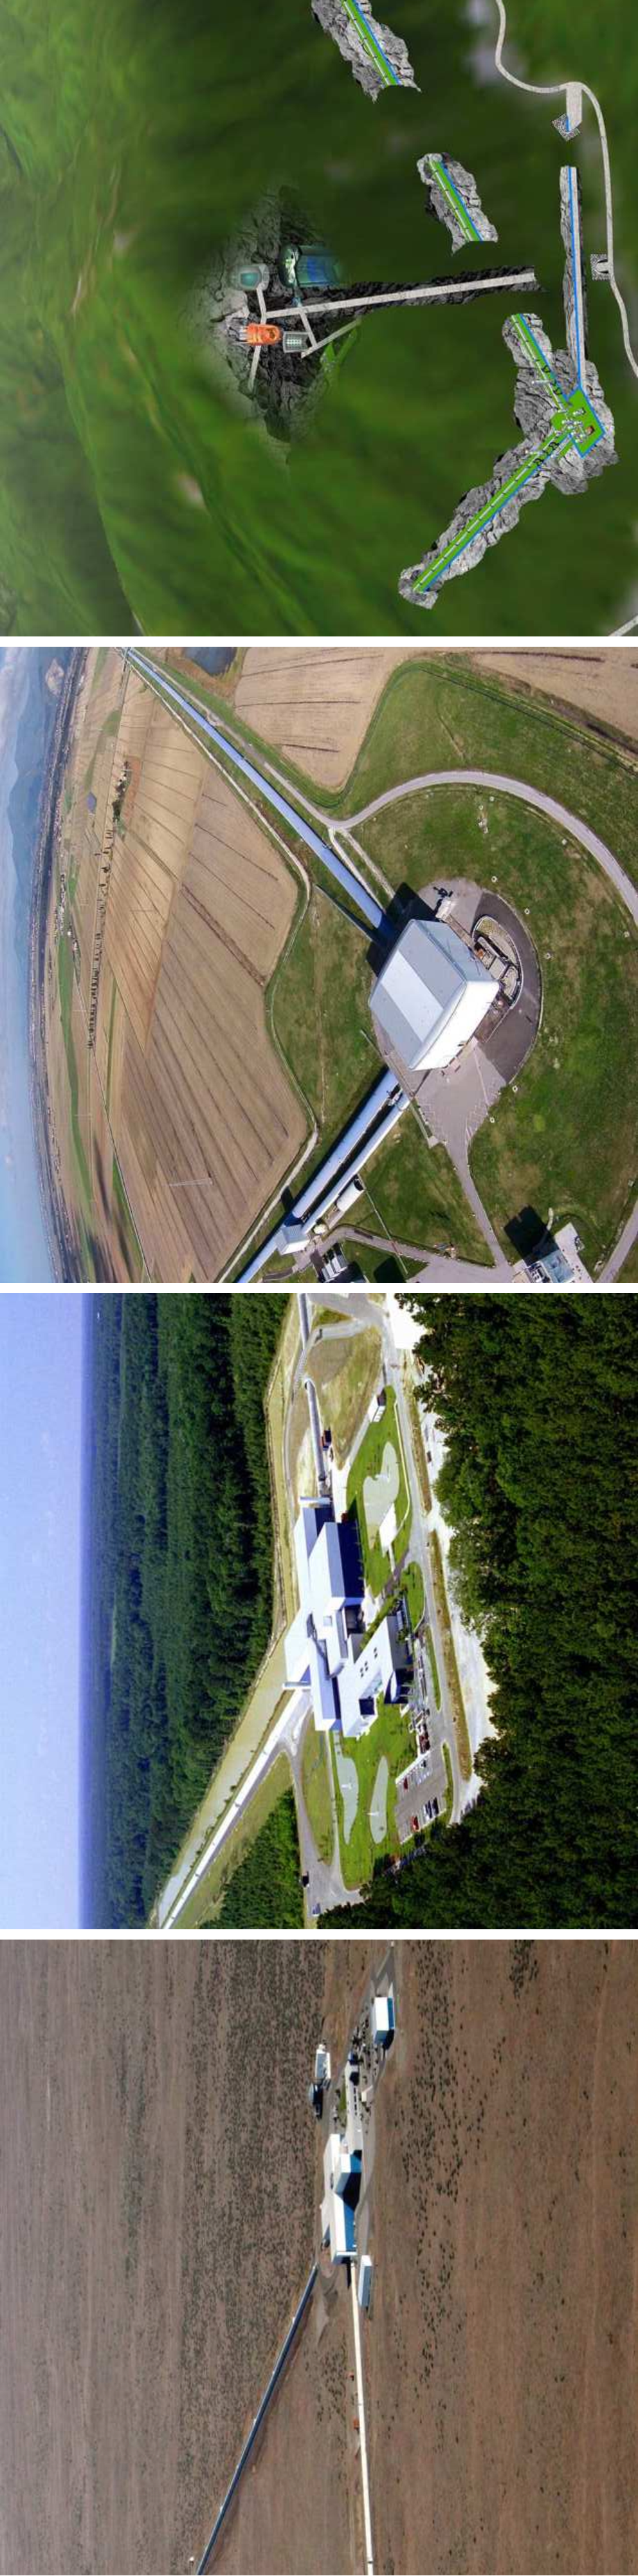
\includegraphics[height=.8\textwidth,angle=-90]{figures/gwo_ifos-pictures.pdf}
	\end{center}
	\caption{Current gravitational wave detectors around the world: LIGO Hanford, LIGO Livingston, VIRGO, KAGRA (left to right). Their interferometer arm lengths are on the order of kilometres. These current detectors are limited in sensitivity at high frequencies (kHz) by quantum noise, which we aim to reduce through internal squeezing.}
	\label{fig:gw_ifos}
\end{figure*}

% gw’s and gw detectors
The first direct detection of gravitational waves in 2015 from the merger of two black holes~\cite{GW150914} opened a new frontier for astronomy. 
Gravitational waves are a prediction of the theory of General Relativity and represent ripples in the ``fabric of space-time'' that stretch and squash the lengths and durations between events. Gravitational wave detectors, including the Advanced Laser Interferometer Gravitational-wave Observatory (aLIGO~\cite{AdvancedLIGO:2015}), are vast and complex experiments that rely fundamentally on the interference of light to detect minuscule changes in the lengths of the two long arms of an interferometer, such as those shown in Fig.~\ref{fig:gw_ifos}. Currently, detectable gravitational waves are limited to come from transient, massive cosmic sources, such as the mergers of binary black holes and neutron stars~\cite{GWTC-1:2018}. With the initial generation of detectors having demonstrated that detection is possible, the natural question now is how to improve upon them to make detectors with higher sensitivity for all kinds of sources.
Possible future sources include continuous gravitational waves from rotating neutron stars~\cite{SuvorovaEtAl:2016}, early universe observations, and higher frequency signals such as those emitted during the late stages of binary neutron star--neutron star mergers.
It is the latter of these sources that concerns us here and so forms our goal of improving the high frequency (kHz) sensitivity of our gravitational wave detectors.


% motivate the need for optical modelling
Due to the complexity of the detectors, deriving analytic solutions for the expected signal and noise output due to a passing gravitational wave is difficult to do, and is impossible to do exactly if we want to include realistic effects. %, and almost never into a closed form. 
While solutions are known for the current configurations, with each new proposed configuration a new set of non-trivial analytics needs to be done. And as the proposals get more exotic the task only grows more tedious.
One solution is to use optical modelling tools that can deliver fast results and let the researcher quickly ascertain the efficacy of a proposed configuration. These optical models also allow the researcher to diagnose the cause of errors in a given detector by selectively including different physical effects in the model.


% what we do
In this report, we demonstrate the use of Finesse~\cite{finesse}, an existing optical modelling software, for a variety of gravitational wave detector configurations and compare against known analytics. In particular, we test the implementation of a non-linear element, a squeezer crystal, in Finesse.
We test this component first in a simple cavity and then in a proposed detector configuration with a squeezer inside of a long signal recycling cavity, this configuration is called ``internal squeezing''.
Current gravitational wave detectors only use a squeezer externally to the interferometer and inject in the squeezed states.
At high frequencies, these detectors are limited by quantum noise, in particular, shot noise. Internal squeezing is predicted to improve the quantum noise limited sensitivity around the coupled cavity pole above the current detectors~\cite{Korobko_2019,Adya_2020}, without increasing the circulating power in the arms nor affecting the low frequency sensitivity of the detector.
By testing internal squeezing in Finesse we can attempt to verify these claims, but first we must demonstrate that we can trust the new implementation to accurately simulate squeezing.


% report structure
This report is structured as follows.
In Section~\ref{sec:Finesse} we detail Finesse and what it does.
In Sections~\ref{sec:basics}~\ref{sec:squeezing} we review the basics of interferometry and squeezing, respectively. In Section~\ref{sec:gwIFO} we detail the aLIGO configuration.
In Section~\ref{sec:sqzcavity} we test the non-linear element in a squeezed cavity against derived analytics in Appendix~\ref{app:squeezed_cavity_analytics}. 
In Section~\ref{sec:aLIGOcomparison} we compare a model of the aLIGO configuration in Finesse to known analytics, with and without internal squeezing, for a variety of interferometer parameters.
We suggest directions for future work in Section~\ref{sec:future_work} and draw conclusions in Section~\ref{sec:conclusions}.


%%%%%%%%%%%%%%%%%%%%%%%%%%%%%%%%%%%%%%%%%%
\section{Finesse} %- Optical modelling
\label{sec:Finesse}
% this section can be quite short

% what does finesse do, how does it do it
Finesse~\cite{finesse} (Frequency domain INterfErometer Simulation SoftwarE) is designed for modelling interferometer configurations (such as those in Section~\ref{sec:gwIFO}). For a specified configuration of optical components, at each connecting node it calculates the amplitudes for the carrier, any control signals, the gravitational wave signal sidebands, and the quantum noise sidebands (see Section~\ref{sec:basics}). By solving the appropriate matrix equations, it does all of this entirely in the frequency domain and therefore in the steady-state regime.
By placing appropriate detectors at the output, Finesse is able to calculate the expected signal and quantum noise transfer functions and so the sensitivity of a proposed detector configuration, which is what we are interested in modelling (see Section~\ref{sec:aLIGOcomparison}). Finesse is actively used for gravitational wave detector commissioning~\cite{brown2020pykat} and outside gravitational wave research for modelling optical cavities.


Although not explored here, Finesse is also able to handle physical effects such as the spatial geometry of Gaussian beams, noise coupling from different parts of the interferometer, imperfections on mirror surfaces, optical misalignment, and higher order modes~\cite{Bond_et_al_2016}. The inclusion of such physical effects means that it can better model and diagnose experiments than with our analytics alone, as the analytics often assume some level of idealisation of the interferometer.


% what is new
Newly implemented in Finesse is a non-linear element component (henceforth \code{nle}) that simulates a squeezer crystal (see Section~\ref{sec:squeezing}). The modelling of this component was based on similar analytics to those in Appendix~\ref{app:squeezed_cavity_analytics}. Unlike the existing squeezer component (e.g.\ \code{sq}), the \code{nle} can be placed anywhere within the configuration. This allows us to model the internal squeezing configuration detailed in Section~\ref{sec:gwIFO}. We are interested in both testing if this component is implemented correctly and in using it to examine proposed detector configurations with internal squeezing. Although, applications of the component are not limited to gravitational wave detector modelling.


% how we use it
We interact with the simulation through a Python~\cite{python} wrapper called PyKat~\cite{brown2020pykat}, in particular, this allows for optimisation routines and plotting do be done in Python in order to find optimal configurations. All of our work is documented and available as open source software at \url{https://github.com/daccordeon/aliveKat}.


%%%%%%%%%%%%%%%%%%%%%%%%%%%%%%%%%%%%%%%%%%
\section{Basics of optics for interferometry}
\label{sec:basics}

\subsection{Phase modulation}
% one paragraph
% phase modulation produces sidebands, mirror motion causes phase modulation

The light in a (gravitational wave) interferometer consists of a carrier at around $\omega_0 \approx 10^{14}$ Hz, control and local oscillators at MHz, and noise from classical and quantum sources across the detection band. Detectable gravitational waves are found with frequencies $\Omega$ between Hz and $10$ kHz. When a gravitational wave passes through the interferometer its effect of stretching or squashing space is akin to the end mirrors in the arms moving back and forth. A moving mirror phase modulates the light incident on it. In the time domain, for a simple sinusoidal carrier $A \cos(\omega_0 t)$ with amplitude $A$ incident on a mirror undergoing small sinusoidal motion at some frequency $\Omega \ll \omega_0$, the reflected light has amplitude $A \cos(\omega_0 t + \delta_m \cos(\Omega t + \phi_m))$ where $\delta_m$ is the modulation depth and $\phi_m$ is the relative phase. To justify the mirror motion being small, given a strain $h(t) \approx 10^{-22}$ from a gravitational wave and an arm length $L \approx 10^3$~m the change in distance is $\Delta L = L h(t) \approx 10^{-19}$ m, far smaller than the radius of a proton ($10^{-15}$ m).


In the frequency domain, taking a Taylor expansion assuming the modulation is weak ($\abs{\delta_m} \ll 1$), the modulation appears as sidebands at $\omega_0 \pm \Omega$, at phase $\pi/2$ ahead of the carrier and amplitude proportional to the modulation depth.
Weak amplitude modulation of the form $A (1 + \delta_m \cos(\Omega t + \phi_m)) \cos(\omega_0 t)$, not considered in depth here, similarly results in faint sidebands at $\omega_0 \pm \Omega$ but in phase with the carrier.


Gravitational waves therefore create weak signal sidebands in the arms of the interferometer. Noise sources (including quantum noise which we consider here) can also shake the mirrors and create their own sidebands of comparable magnitude in the same frequency range. Measuring the signal sidebands despite the noise is the role of the rest of the detector, see Section~\ref{sec:squeezing}.


\subsection{Types of optical cavities}
% one paragraph
% interference of reflected field and circulating field
% Coupled, overcoupled, undercoupled

\begin{figure}[h]
	\begin{center}
	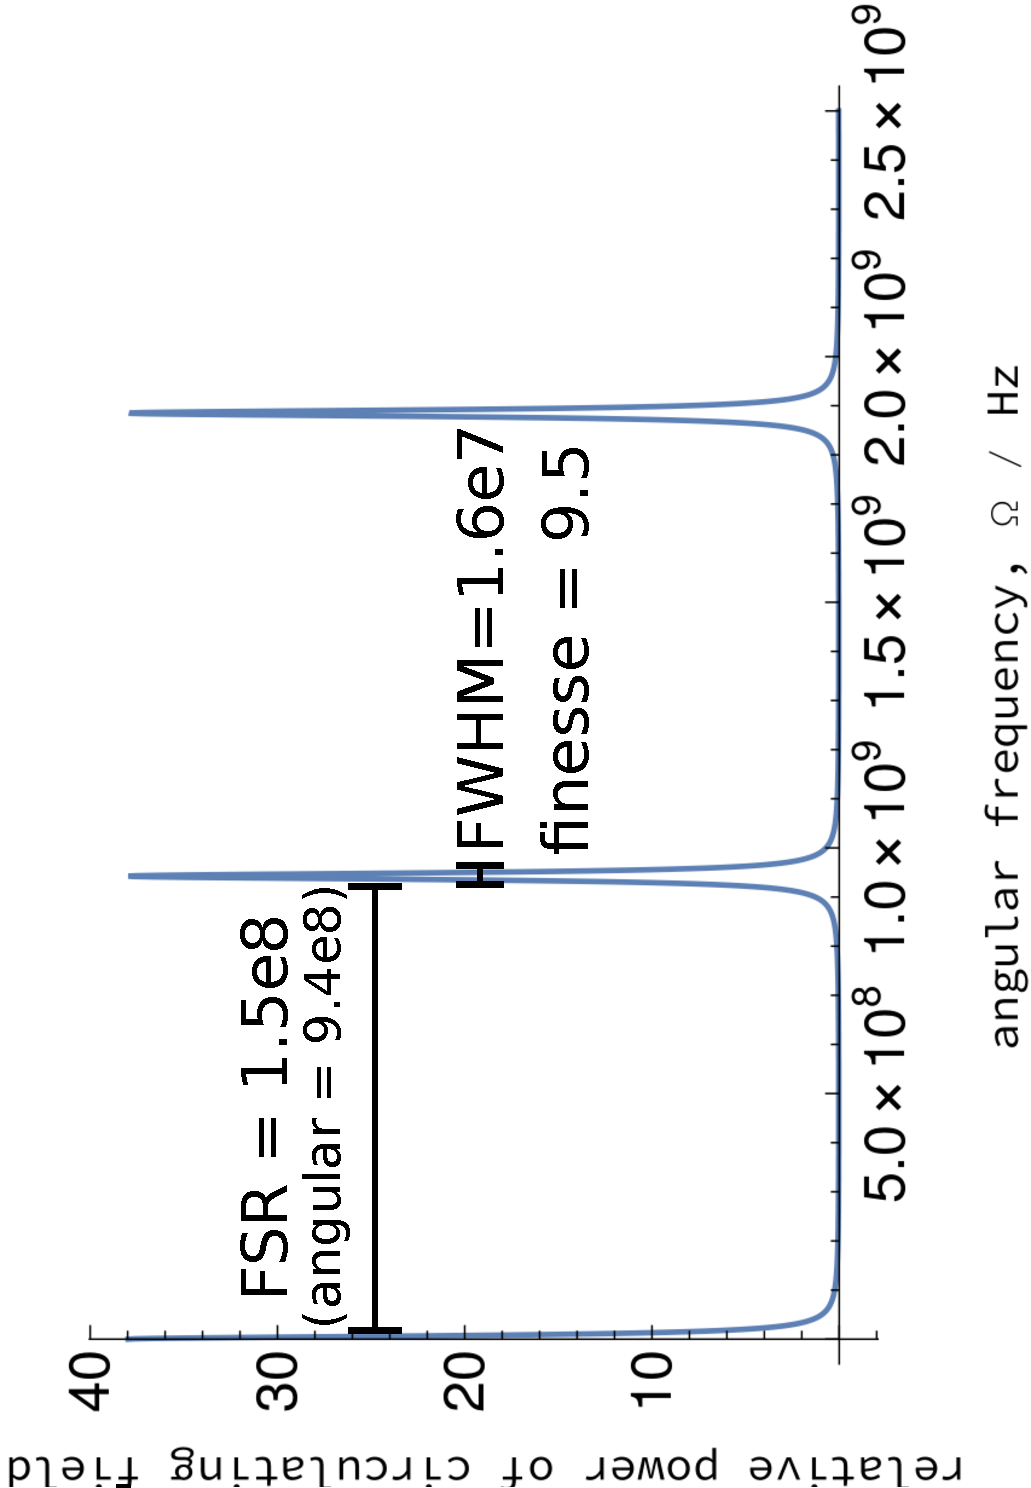
\includegraphics[height=0.45\textwidth, angle=-90]{figures/cavity_fsr_fwhm_finesse.pdf}
	\end{center}
	\caption{Circulating power in an overcoupled cavity relative to incident power, generated by analytics. Cavity of length 1 m and with reflectivities $r_1 = 0.9^{1/2}$ and $r_2 = 1$ for the front and back lossless mirrors, respectively. Showing the FSR, FWHM, and finesse of the cavity. We will use the FSR later to test the implementation of a non-linear element in Finesse.}
	\label{fig:cavity_fsr_fwhm_finesse}
\end{figure}

In gravitational wave detectors many cavities are used to perform a variety of functions, see Section~\ref{sec:gwIFO}. Any cavity is equivalent to a two mirror cavity. Consider two lossless mirrors with reflectivities $r_1$ and $r_2$ separated by a space of macroscopic length $L$. Meaning that it is tuned to the wavelength $\lambda$ of the light and is actually of length $\lfloor \frac{L}{\lambda} \rfloor \lambda$. Of the light incident on mirror 1 from outside the cavity, $\abs{r_1}^2$ of the power is reflected directly off and undergoes no phase change (using the convention of no phase change on reflection and $\pi/2$ on transmission). The light that enters the cavity will either continue to circulate or eventually leave through either mirror. The circulating light that eventually leaks back out through mirror 1 has undergone a phase change of $\pi$ and so will destructively interfere with the directly reflected light. The result of this is that the power ratio of the incident to the reflected light, by working in the frequency domain, is given by~\cite{Danilishin_2012}
$$\abs{\frac{E_{\mathrm{refl}}}{E_{\mathrm{inci}}}}^2 = \abs{\frac{r_1 - r_2 e^{-i 2 L \frac{2\pi}{\lambda}}}{1- r_1 r_2 e^{-i 2 L \frac{2\pi}{\lambda}}}}^2.$$ 

The result of which is that Fabry-Peroy cavities (the ones we’re studying here) fall into three categories determined by which of the two reflected fields dominate, which depends on the relative size of $r_1$ and $r_2$. If $r_1 = r_2$ then the cavity is impedance matched, the fields exactly balance and no light is reflected back. If $r_1 < r_2$ then the cavity is overcoupled, the transmitted circulating fields wins out and light is reflected off the cavity at a $\pi$ phase shift. And if $r_1 > r_2$ then the cavity is undercoupled, the directly reflected field wins out and the light is reflected back at the same phase it came in at. In gravitational wave detectors both overcoupled cavities (e.g.\ the arm cavities) and impedance matched cavities (e.g.\ the power recycling cavity, when no reflection is necessary) are used.


If the reflectivies are fixed and instead the frequency of the incoming light is changed, then resonance peaks are seen in the power of the circulating field whenever the roundtrip distance is some multiple of the wavelength. The distance between these peaks, the free spectral range (FSR), is therefore given by $$\mathrm{FSR} = \frac{c}{2L}.$$ Comparing this to the full-width at half-maximum (FWHM) of each peak (also known as the linewidth) gives a dimensionless rating for the cavity that allows for different cavities to be compared, the finesse (cf.\ the quality factor of an oscillator) $$\mathrm{finesse} = \frac{\mathrm{FSR}}{\mathrm{FWHM}}.$$
The FSR, FWHM, and finesse of an example overcoupled cavity are shown in Figure~\ref{fig:cavity_fsr_fwhm_finesse}.
For reference, the aLIGO arm cavities have a finesse of $440$~\cite{AdvancedLIGO:2015} compared to the finesse of $9.5$ shown.


\section{Generation and detection of squeezed states}
\label{sec:squeezing}

\begin{figure}[ht]%
	\begin{center}
	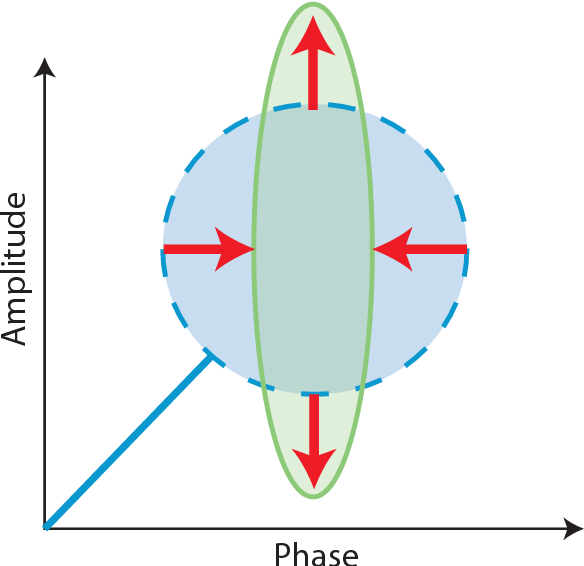
\includegraphics[width=0.3\textwidth]{figures/ball_and_stick_squeezed_state.png}
	\end{center}
	\caption{Ball and stick figure of a squeezed coherent state in amplitude/phase space. The stick represents the DC amplitude of the state (zero length for a vacuum state, which is centred on the origin). The dashed blue noise circle represents the unsqueezed state with symmetric uncertainty in amplitude and phase. The green noise ellipse represents the state after squeezing in phase (red arrows show direction of squeezing). The area of the two shapes should be equal. Figure taken from Ref.~\cite{Sparkes2013StorageAM} (without permission).}
	\label{fig:ball_and_stick_squeezed_state}
\end{figure}

\subsection{Squeezed states}
% one paragraph

Given a sinusoidal signal, one can decompose it into two quadratures $A_C \cos(\Omega t) + A_S \sin(\Omega t)$, called the cosine and sine or the amplitude and phase quadratures (so called because of the effects of amplitude and phase modulation being seen in their respective quadratures). Note that the quadrature decomposition of all the light in the interferometer is relative and taken (typically) with respect to the carrier.


We are interested in quadratures because they lead to a simple explanation of squeezing. In the quantum mechanical two-photon formalism~\cite{Danilishin_2012}, the quadratures relate the harmonic oscillator creation/annihilation operators of the sidebands ($\hat{a}_{\omega_0 \pm \Omega}^\dagger, \hat{a}_{\omega_0 \pm \Omega}$) around the carrier. Assuming that $\Omega \ll \omega_0$, these are related by
\begin{align*}
\hat{a}_c(\Omega) &\approx \frac{1}{\sqrt{2}} (\hat{a}_{\omega_0 + \Omega} + \hat{a}_{\omega_0 - \Omega}^\dagger),\\
\hat{a}_s(\Omega) &\approx \frac{1}{i \sqrt{2}} (\hat{a}_{\omega_0 + \Omega} - \hat{a}_{\omega_0 - \Omega}^\dagger).
\end{align*}
In quantum optics, these then define dimensionless “position” and “momentum” operators $\hat{X}, \hat{Y}$, the moments of which describe the uncertainty in each quadrature (and are also equal to values in the spectral density and covariance matrices~\cite{Danilishin_2012}). These uncertainties are equivalent to uncertainty in the amplitude and phase of the electric field.


Consider a vacuum state, although the expected value for either quadrature is zero $\langle \hat{X} \rangle = \langle \hat{Y} \rangle = 0$, due to the Heisenberg Uncertainty Principle (HUP) the standard deviations are limited by $\mathrm{Var}[\hat{X}]^{1/2} \mathrm{Var}[\hat{Y}]^{1/2} \geq 1/2$. Imagining the distribution of the state in $X \times Y$ phase space, this means that smallest area the noise ellipse corresponding to one standard deviation can have is $1/2$. The vacuum ground state with minimum uncertainty has equal radii of $1/\sqrt{2}$.


Squeezing a state simply scales one quadrature variance down by some factor while scaling the other quadrature variance up by the same factor, as to maintain the HUP. In phase space, this looks like squeezing (hence the name) the noise circle: one of its radii decrease and the other increases such that the area remains the same, as shown in Figure~\ref{fig:ball_and_stick_squeezed_state}. A squeezer requires two parameters, the squeezing strength $r_{\mathrm{dB}} = 20 \log_{10}(e^r)$ and the squeezing angle $\phi_{\mathrm{sqz}}$. The squeezing strength measures, in dB, the gain in the squeezed quadrature. For a squeezed (vacuum) state the radii get scaled to $e^{\pm r}/\sqrt{2}$. The squeezing angle determines along which line the noise ellipse is squeezed.

\subsubsection{Spectral density}

% spectral density of the quantum noise
The goal of squeezing in a gravitational wave interferometer is primarily to control the quantum noise in a given quadrature. By squeezing the vacuum input (see Section~\ref{sec:gwIFO}) we change the spectrum of the quantum noise, reducing the noise in one quadrature while worsening it in the other. The (double-sided) power spectral density (PSD) $\hat{S}_Z$ of the quantum noise $\hat{Z}$, given a spectrum $\hat{Z}(\Omega)$, is given by $$\hat{S}_Z(\Omega) 2 \pi \delta(\Omega - \Omega') = \langle0| \hat{Z}(\Omega) \circ \hat{Z}^\dagger(\Omega') |0\rangle$$ where $|0\rangle$ is the vacuum state and $\circ$ is the symmetric product $A \circ B = \frac{1}{2}(A B + B A)$.

Note that the convention for strain sensitivity uses amplitude spectral density (ASD), e.g.\ lossless 6 dB of injected external squeezing improves the quantum noise limited strain sensitivity measured as ASD by a factor of 2~\cite{Aasi_2013}.
Therefore, the convention for dB is defined as $20 \log_{10}(Q/{Q(0)})$ for some quantity $Q$.

\subsection{Generation of squeezed states}

\begin{figure}[ht]%
    \centering
    \subfloat[\centering ]{{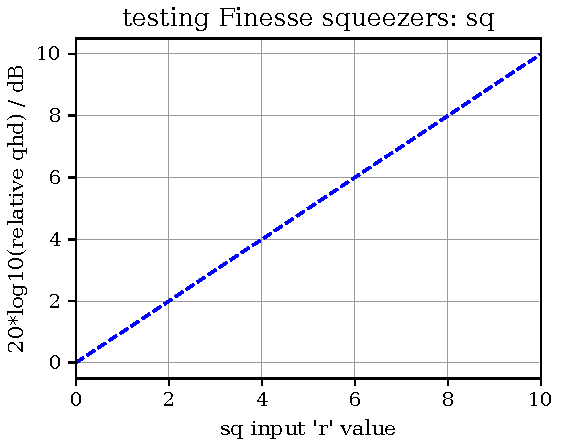
\includegraphics[width=0.3\textwidth]{figures/testing_Finesse_squeezers-sq.pdf}}}%
    \\
    \subfloat[\centering ]{{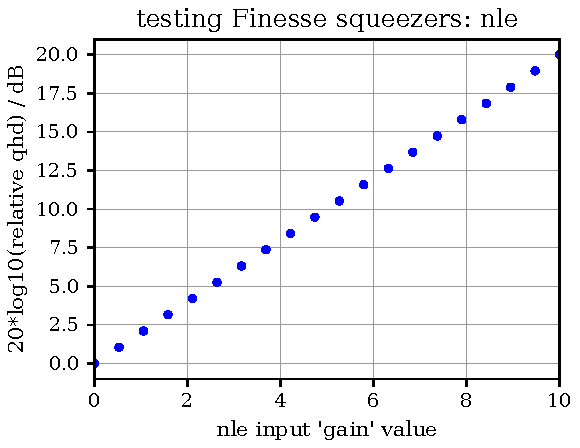
\includegraphics[width=0.31\textwidth]{figures/testing_Finesse_squeezers-nle.pdf}}}%
    \caption{Basic comparison of squeezers implemented in Finesse. Comparing the dB gain (using the $20 \log_{10}$ convention) in the squeezed quadrature versus the input squeezer parameter, for \code{sq} in panel~a~(top panel) and \code{nle} in panel~b~(bottom panel). This figure shows that \code{nle} gains by a factor of two more than convention.}%
    \label{fig:testing_Finesse_squeezers}%
\end{figure}

In the laboratory (or in a gravitational wave detector like aLIGO), squeezed states are generated in a non-linear crystal in which parametric down conversion (PDC) occurs stimulated by a pump laser. In degenerate squeezing, a photon of pump frequency $2\omega_0$ is annihilated and two photons of frequency $\omega_0$ are created (called the signal and the idler). The non-linear crystal is designed to be directional in that squeezing occurs if the light passes in one direction through the crystal but in the other direction the light is unaffected.


In the analytics used here, squeezing is performed by suitable multiplication of the quadrature amplitudes by a squeezing matrix. Given a squeezer parameter $r$ as input, the squeezing strength (or, the amount of signal gain) in dB is given by $r_{\mathrm{dB}} = 20 \log_{10}(e^r)$. The analytics also accounts for the directionality of the squeezer crystal.


In the non-linear element (\code{nle}) implementation in Finesse, squeezing is performed by similar quadrature manipulation as the analytics. Given a gain value in dB as input, the \code{nle} will produce twice that amount of squeezing as output. In other words, the \code{nle} treats the dB input as $10 \log_{10} (e^r)$ (a power quantity) instead of $20 \log_{10} (e^r)$ (an amplitude quantity) as in the convention mentioned above. This can be seen in Fig.~\ref{fig:testing_Finesse_squeezers}, the right panel displays the \code{nle} while the left panel displays the other, external squeezer component (\code{sq}) which behaves conventionally. Additionally, the \code{nle} will squeeze states incident from either side, it is direction-less. These differences will be apparent in the results shown, see Sections~\ref{sec:sqzcavity}~\ref{sec:aLIGOcomparison}.


\subsection{Homodyne readout}
% one paragraph

To detect the faint signal sidebands we use a readout scheme. In homodyne readout, the signal is mixed with a strong local oscillator at a beamsplitter. The local oscillator comes from a second laser at the carrier frequency $\omega_0$ but with some relative phase to the carrier, called the homodyne angle $\phi_{\mathrm{LO}}$. After the beamsplitter, the two mixed beams, with different relative phases between the signal and local oscillator, are each read by a photodiode.
The resultant homodyne current is proportional to the difference in intensities at the photodiodes.
Homodyne readout in a simplified aLIGO configuration is shown inside the dashed blue box in Fig.~\ref{fig:aLIGO_configuration}.


The homodyne current is proportional to the amplitude of the local oscillator times a combination of the sideband quadrature amplitudes dependent on $\phi_{\mathrm{LO}}$, yet is independent of any laser noise from the local oscillator. Appropriate choice of $\phi_{\mathrm{LO}}$ allows the squeezed quadrature to be extracted. Note that homodyne readout does nothing to reduce the noise in the sidebands, it just allows for the benefits of squeezing to be gained by filtering out the anti-squeezed (or worsened) quadrature.


%%%%%%%%%%%%%%%%%%%%%%%%%%%%%%%%%%%%%%%%%%
\section{Gravitational wave detector interferometry}
\label{sec:gwIFO}

\subsection{The Michelson interferometer}
% one paragraph

\begin{figure}[ht]
	\begin{center}
	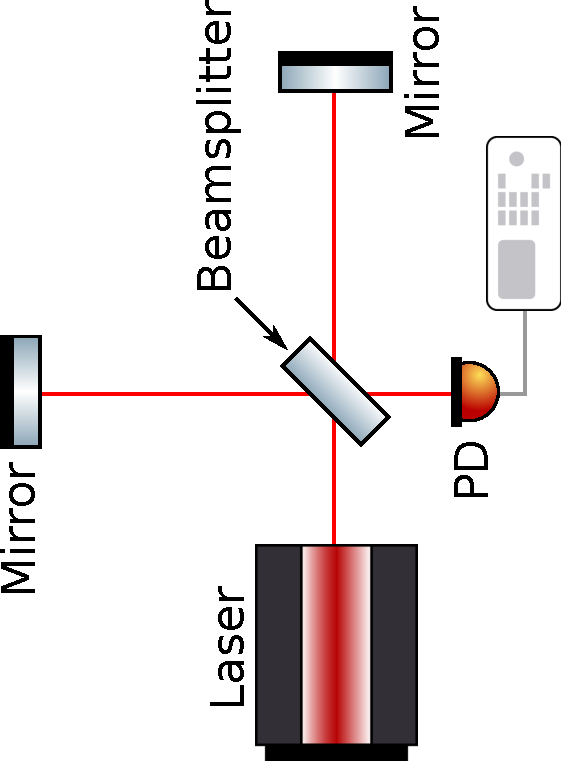
\includegraphics[width=0.35\textwidth]{figures/Michelson_interferometer.pdf}
	\end{center}
	\caption{Configuration of a simple Michelson interferometer. A laser beam is split down two arms, reflects off a mirror at the end of each arm, and then interferes back at the beamsplitter. At the output of the beamsplitter a photodiode is placed to read any amplitude modulation due to phase modulation in the arms.}
	\label{fig:Michelson}
\end{figure}

In its simplest form (ignoring spatial effects henceforth), a Michelson interferometer consists of a laser, a beamsplitter, two arm mirrors, and a photodiode. The laser light is split and travels down two arms, reflects off a mirror at the end of each arm, and then recombines at the beamsplitter output, at which a photodiode is placed. The differential length of the two arms produces interference at the beamsplitter.
If something perturbs the mirrors (e.g.\ a gravitational wave or some noise) and creates phase modulation of the carrier in the arms, then the interference at the beamsplitter converts that modulation to amplitude modulation, which can be detected at the photodiode.


By tuning the unperturbed lengths of the arms, the output of the beamsplitter can be made such that, by default, no carrier is present. This is known as setting the output to the darkport or as setting the operating point of the interferometer to a dark fringe. In practise, the operating point is set slightly off the dark fringe to balance the response to the differential length change and the amplitude of the sidebands.


In the farfield, a gravitational wave stretches and squashes the distances between objects in a quadrupole manner. Transverse to the axis of propagation distances in one direction are stretched while those in the perpendicular direction are squashed. In order to best detect these changes we need two pairs of objects at right angles to each other (and, ideally, to the gravitational wave). These pairs consist of each mirror and the beamsplitter.


\subsection{Configuration of aLIGO}
% (not investigated here): external squeezing, mode cleaning and spatial effects

\begin{figure}[ht]
	\begin{center}
	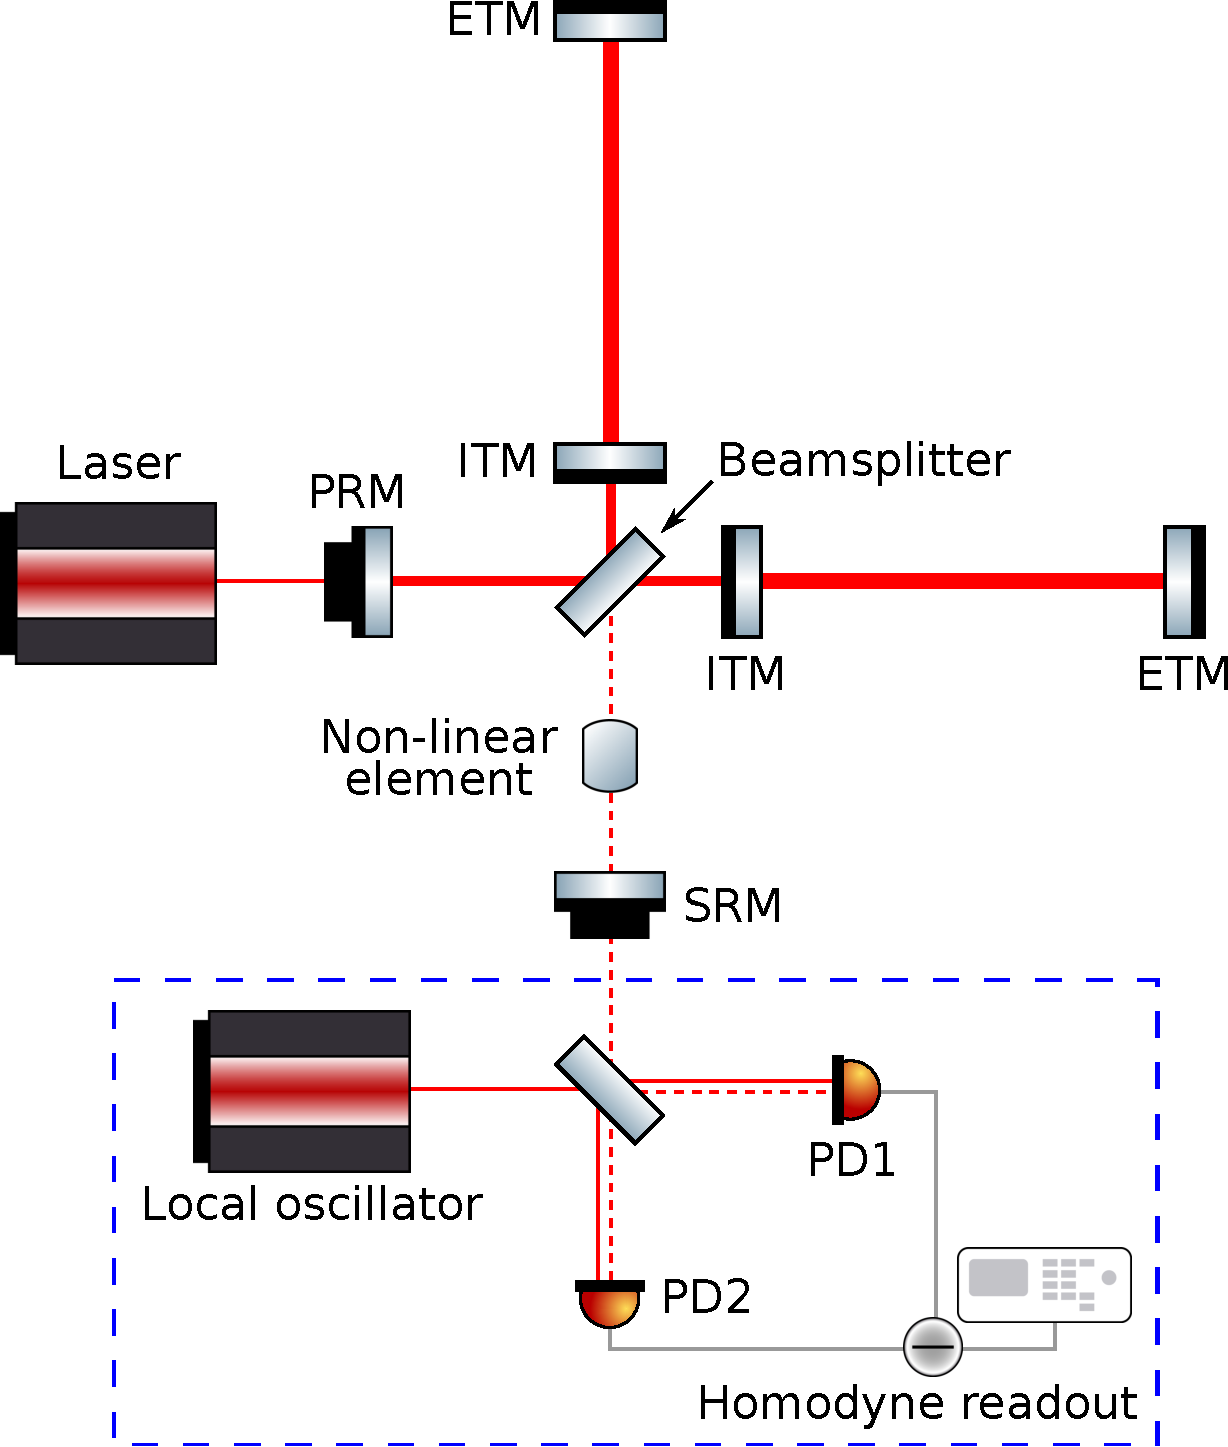
\includegraphics[width=0.45\textwidth]{figures/aLIGO_internal_squeezing.pdf}
	\end{center}
	\caption{Simplified configuration of aLIGO with internal squeezing. Building on the Michelson interferometer in Fig.~\ref{fig:Michelson}, this configuration adds in arm cavities (between ITM and ETM), a power recycling mirror (PRM), and a signal recycling mirror (SRM) all to improve the sensitivity of the detector by boosting the power in the arms or the time that the signal spends there. A non-linear element is placed in a long SRC to perform internal squeezing. Readout of the signal and noise is done via balanced homodyne readout, shown in the dashed blue box.}
	\label{fig:aLIGO_configuration}
\end{figure}

We study a simplified aLIGO configuration, shown in Fig.~\ref{fig:aLIGO_configuration}, and provide motivation for each component.


% arm cavities, prc, src, 
To achieve the sensitivity required for gravitational wave detection, a classical Michelson interferometer requires technically infeasible amounts of power in the arms in order to reduce the shot noise, see Section~\ref{sec:noise_sources}, and arm lengths tens of kilometres long.
The effective arm length can be increased by increasing the storage time in the arms, i.e.\ by making the light experience the gravitational wave’s effects for longer. This is achieved by introducing another mirror into each of the beam arms, forming an overcoupled arm cavity between an initial test mass (ITM) and an end test mass (ETM) (in aLIGO each are 40 kg heavy and made of fused silica~\cite{AdvancedLIGO:2015}). The circulating power in the arm cavities is also far higher and so reduces the shot noise.


To further increase the power in the arms, a power recycling mirror (PRM) is introduced before the beamsplitter, this reflects power returning from the arm cavities back into the interferometer. For reference, in aLIGO a $125$ W laser results in $\approx 5$ kW of power incident on the beamsplitter and beyond $600$ kW of power in the arms.


For a passing gravitational wave to result in detectable changes in the arm lengths, the beam arms need to be at least kilometres long (e.g.\ $4$ km long in aLIGO). To increase sensitivity, the signal from the darkport of the beamsplitter can be amplified by reflecting it back into the arms to ``see'' the gravitational wave again. This is done by placing a signal recycling mirror (SRM) after the darkport of the beamsplitter. What the signal recycling cavity (SRC) actually does is more complicated, see Section~\ref{sec:long_srcs}.


\subsubsection{Reduction of aLIGO to coupled cavities}
% simplification to coupled cavities

\begin{figure}[ht]
	\begin{center}
	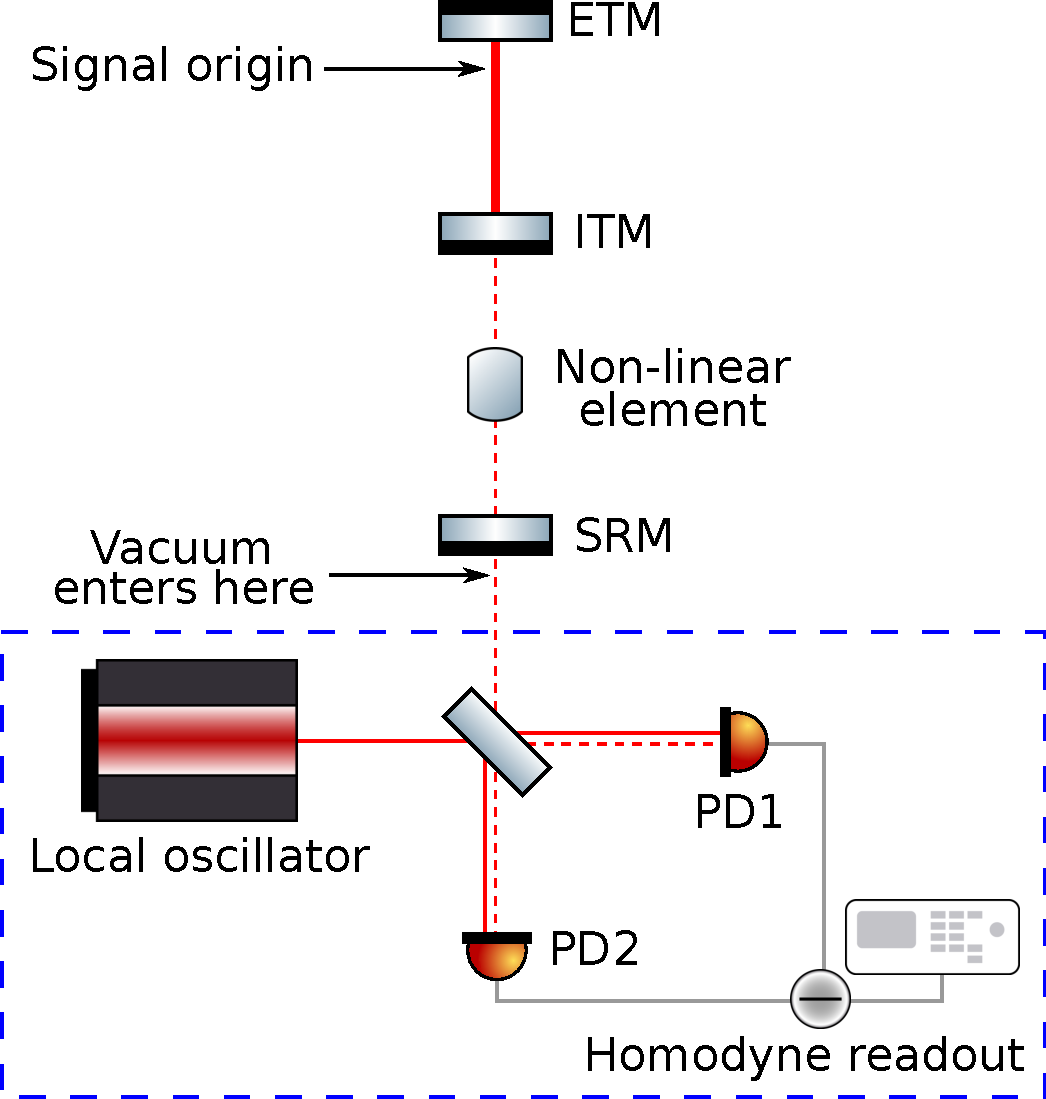
\includegraphics[width=0.4\textwidth]{figures/aLIGO_as_coupled_cavities.pdf}
	\end{center}
	\caption{Reduced configuration of aLIGO from that shown in Fig.~\ref{fig:aLIGO_configuration} to two coupled cavities representing the SRC and the arm cavities. This reduction holds to a great approximation. The benefit of the reduction is to realise how the signal and the vacuum fluctuations see the non-linear element differently since the enter from different sides of the interferometer.}
	\label{fig:aLIGO_as_coupled_cavities}
\end{figure}

Despite all the components in the (simplified) aLIGO, the resultant transfer functions for the signal and the noise are equivalent (to a good approximation) to those for two coupled cavities, shown in Fig.~\ref{fig:aLIGO_as_coupled_cavities}. The differential mode from the two arms becomes an optomechanical coupling between the SRC and the beam arm.
Although the coupled cavity system isn’t physical, for example the source of the laser in arm cavity is non-existent, the reduction is useful to understanding the interferometer. In particular, it is clear in the reduced system that the signal and the vacuum fluctuations see the cavities differently as they they enter from different sides. This explains how internal squeezing can affect them differently, as discussed in Section~\ref{sec:internal_squeezing}.


\subsection{Noise sources}
\label{sec:noise_sources}
% strain plot, quantum noise limited strain sensitivity
% quantum, Newtonian (seismic), thermal,

\begin{figure*}[ht]%
	\begin{center}
	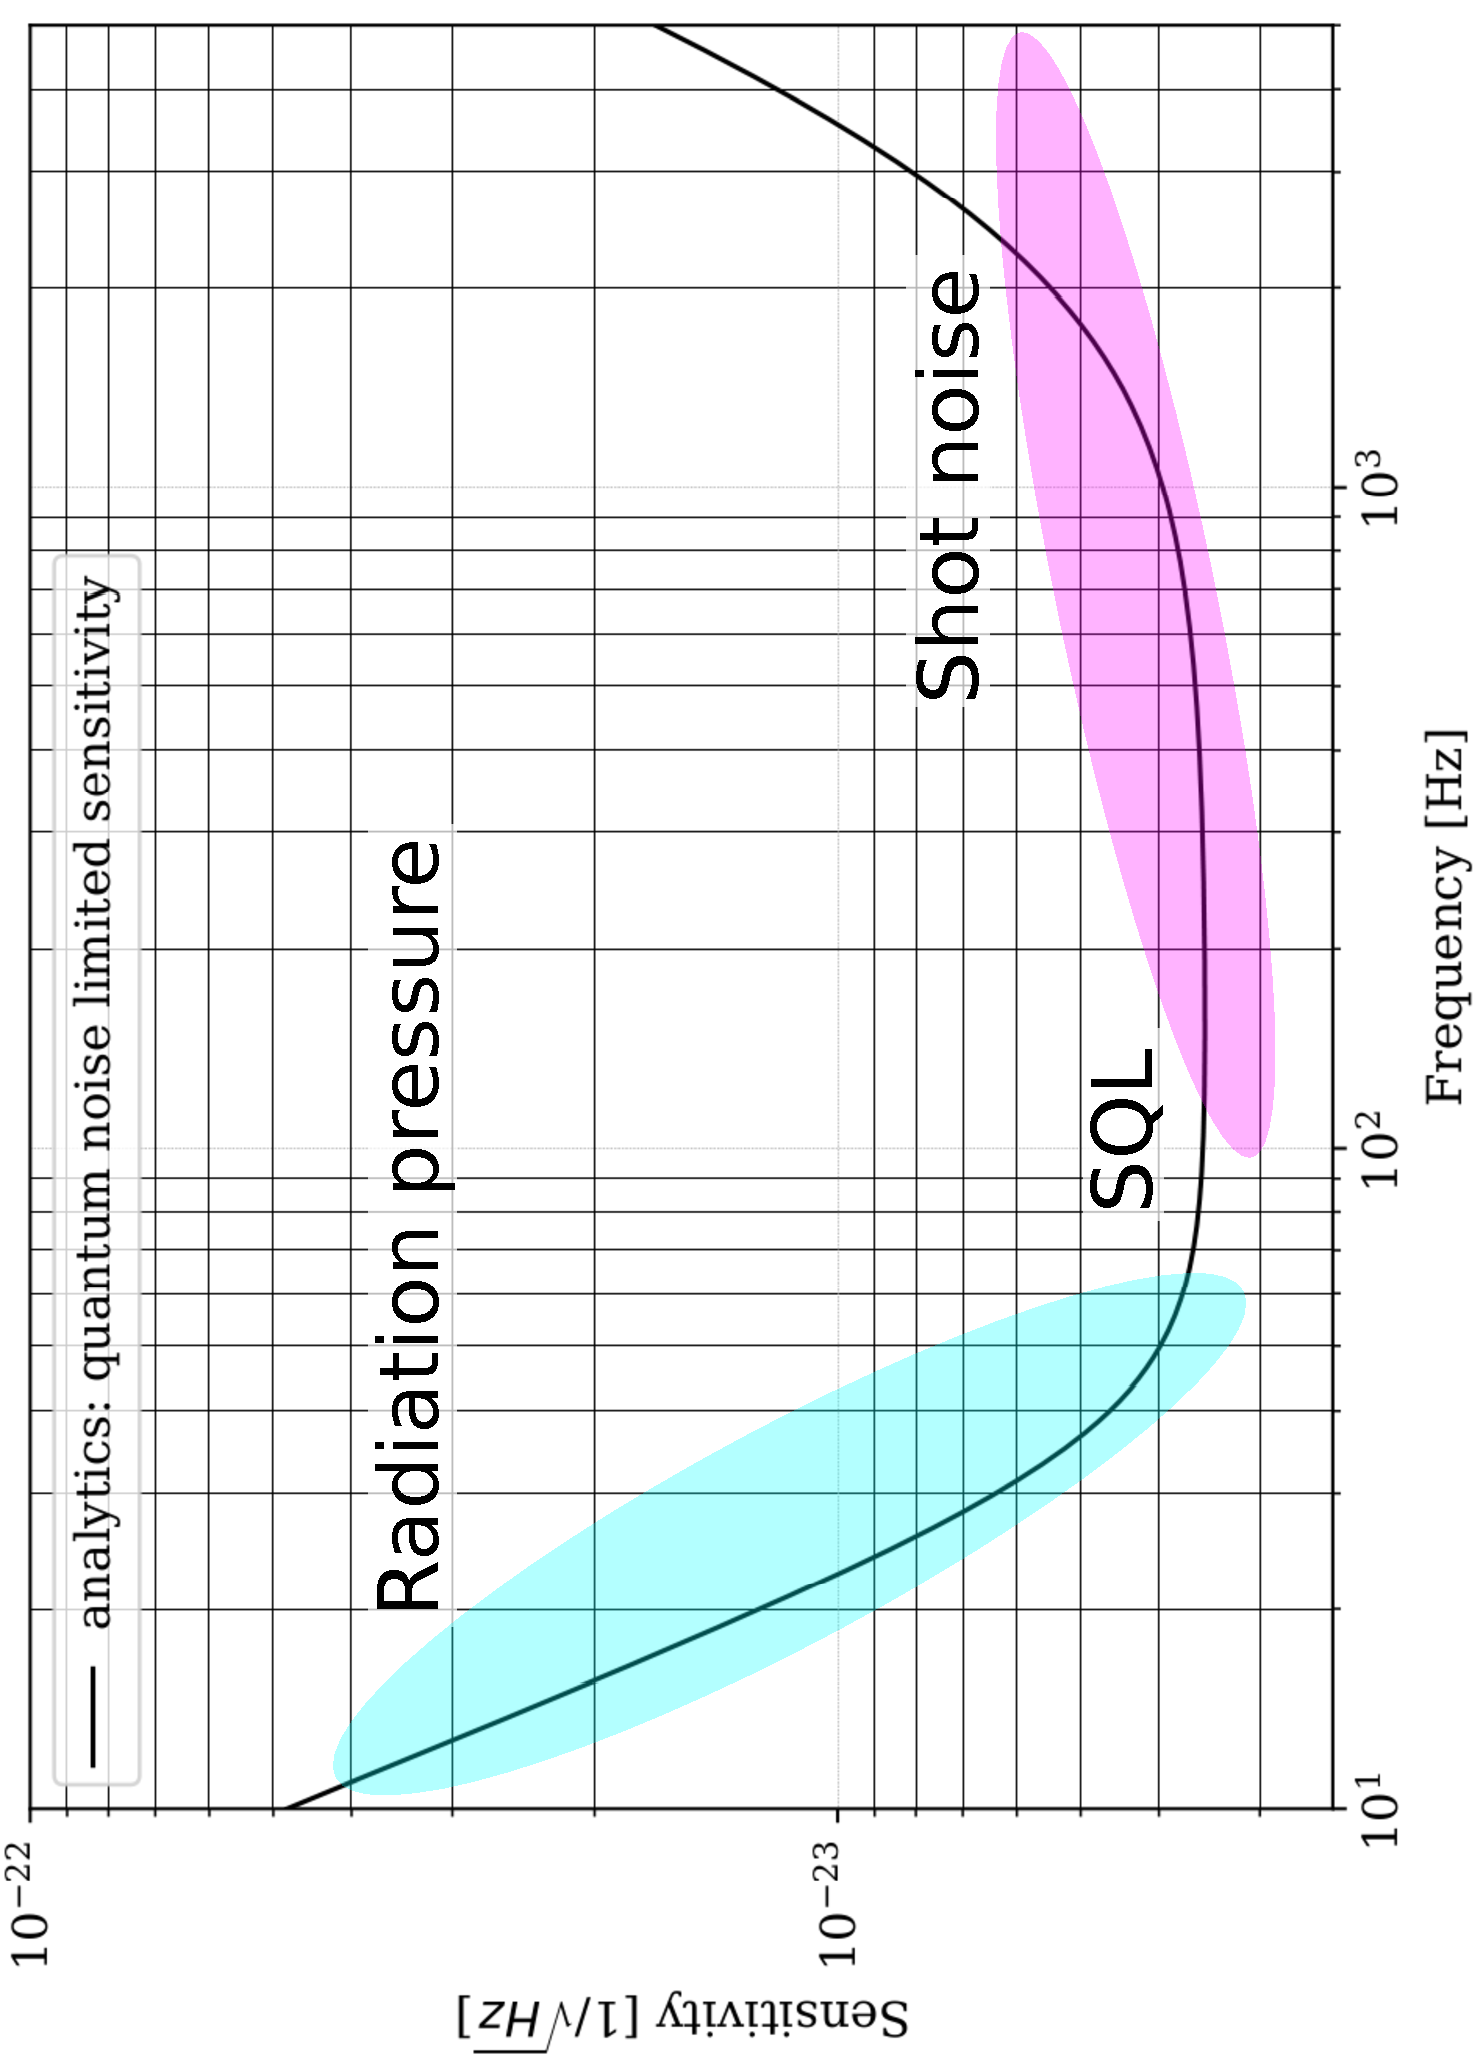
\includegraphics[width=0.6\textwidth]{figures/sqz_aLIGO_analytics_quantum_noise_budget-labelled.pdf}
	\end{center}
	\caption{Quantum noise limited sensitivity of aLIGO (shown without any squeezing). This figure was generated using existing analytics. This figure shows the regions where the radiation pressure (blue) or the shot noise (pink) dominates, along with the standard quantum limit (SQL) where they balance. At high frequencies, the shot noise dominates and we aim to reduce it via internal squeezing.}
	\label{fig:sqz_aLIGO_analytics_quantum_noise_budget}
\end{figure*}


In aLIGO, noise enters the system from many sources and reduces sensitivity across the frequency range of Hz to kHz. Classically, these range from vibrations in the ground (seismic noise) and changing in the nearby distribution of matter (Newtonian noise), to thermal vibration of the components and the space they hang in (thermal noise). Control systems and the natural resonances of the mirror suspensions also remove the possibility for detection in certain bands. We don’t consider these effects here, instead focusing on the quantum noise. We assume that all these noise sources are static in frequency, an often reasonable assumption. 


Quantum noise comes from the fundamental HUP limits on the uncertainty in each quadrature, discussed in Section~\ref{sec:squeezing}. Vacuum enters the interferometer at every open port, most importantly from behind the SRM, and, due to the Fluctuation Dissipation Theorem~\cite{Danilishin_2012}, at every lossy optical component in the form of new, un-correlated noise. In the phase quadrature, quantum noise manifests as shot noise, uncertainty in the number of photons hitting one of the mirrors, that is strongest at high frequencies. In the amplitude quadrature, quantum noise comes as radiation pressure, driving of mirror oscillations by incident light, that is strongest at low frequencies. Increasing the power in the arms reduces shot noise but increases radiation pressure, leading to a trade-off in how much power is put into the interferometer.


To compare the effect of noise sources on the detector’s ability to detect gravitational waves, we define the noise limited strain sensitivity to be the signal amplitude required to achieve a signal-to-noise (SNR) ratio of one, with respect to the given noise source in isolation. This means computing the signal and noise transfer functions for the interferometer and suitably dividing them. The total sensitivity of the interferometer is the SNR with respect to the total noise, equal to the root sum squared of the contribution from each noise source, e.g.\
$$\mathrm{total\; noise = \sqrt{(quantum \; noise)^2 + (thermal \; noise)^2 + \ldots}}$$
In frequency, the maximum sensitivity with respect to quantum noise is achieved where the radiation pressure and shot noise balance, known as the standard quantum limit (SQL), shown in Fig.~\ref{fig:sqz_aLIGO_analytics_quantum_noise_budget}. Recall from Section~\ref{sec:introduction} that current gravitational wave detectors are limited at high frequencies by shot noise and so improvement of high frequency sensitivity is equivalent to improvement of high frequency quantum noise limited sensitivity, which is what we are aiming to demonstrate here.


\subsection{Short versus long signal recycling cavities}
\label{sec:long_srcs}

\begin{figure*}
	\begin{center}
	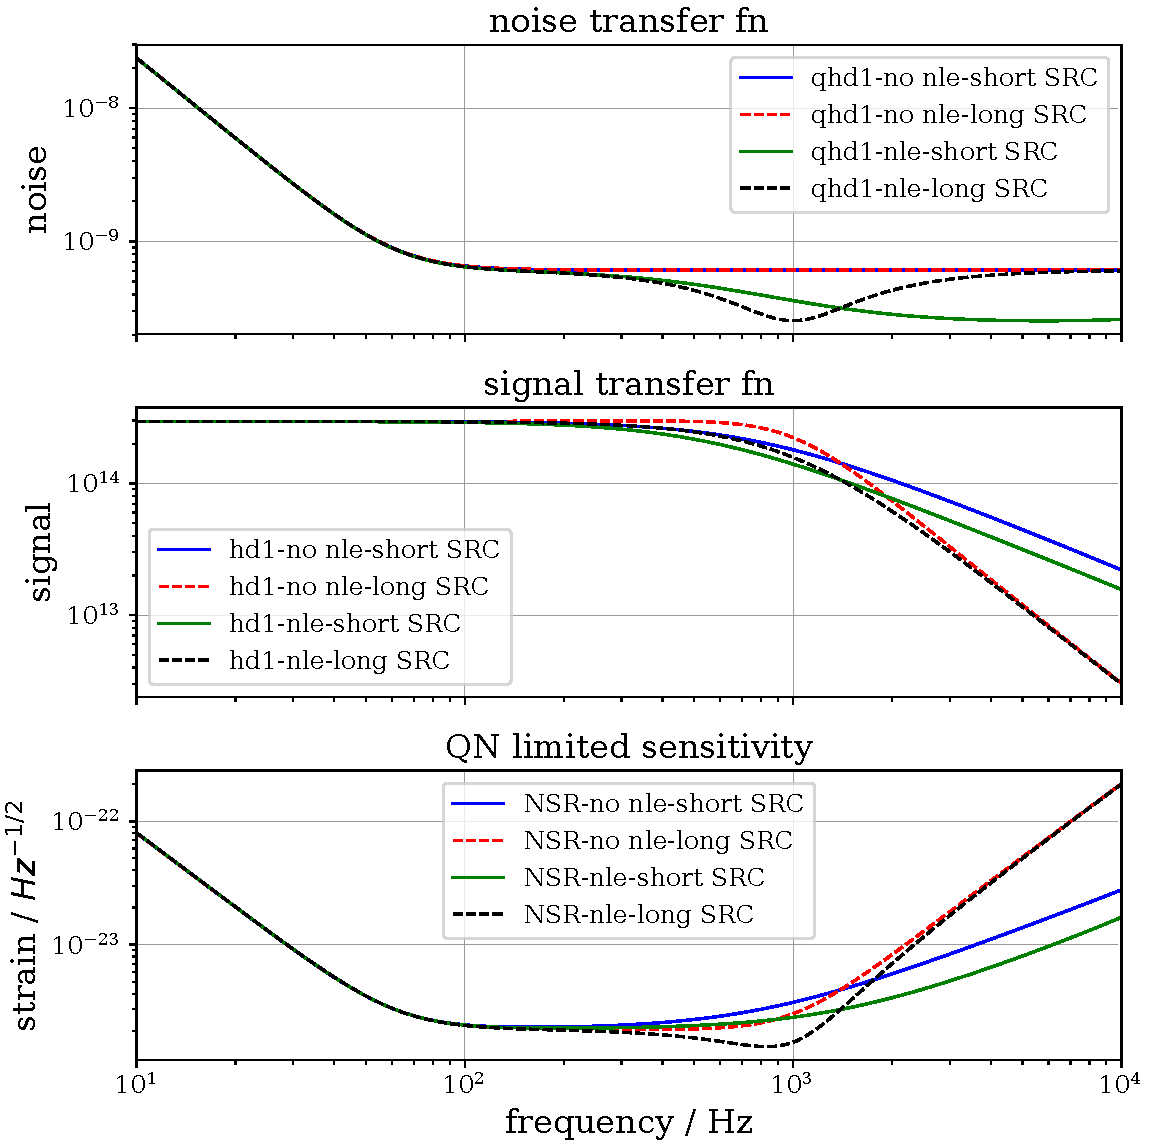
\includegraphics[width=0.6\textwidth]{figures/aLIGO_transfer_fns_and_sensitivity_comparison.pdf}
	\end{center}
	\caption{The quantum noise (top panel), signal transfer function (middle panel), and quantum noise limited strain sensitivity (bottom panel) for aLIGO. This figure shows the results from a model in Finesse for different lengths of SRC (53 m and 2000 m) and with and without internal squeezing. The detectors in Finesse (\code{qhd} and \code{hd}) measure amplitude spectral density (ASD). This figure shows that increasing the length of the SRC increases the peak sensitivity at the coupled cavity pole, decreases the bandwidth after the coupled cavity pole, and changes the frequency band squeezed by the non-linear element. Internal squeezing reduces the quantum noise in a high frequency band, de-amplifies the signal, and results in greater peak sensitivity around the coupled cavity pole. No change is seen in any case at low frequencies.}
	\label{fig:src_transfer_functions}
\end{figure*}

The signal recycling cavity (SRC) amplifies the gravitational wave signal by reflecting it back into the interferometer, as described above.
% Introduction of the SRC also broadens the FHWM of the cavity reasonance.
Considering the coupled cavity system in analogy to a system of two coupled harmonic oscillators (e.g.\ two pendulums connected by a spring), changing the length of the SRC (and/or the transmitivity of the ITM) affects the coupling between the cavities, or the energy transfer between the oscillators. The lowest resonance of the coupled system, known as the coupled cavity pole, is the most sensitive band of the detector. The sensitivity depth and bandwidth of the detector around the pole depend on the parameters of the SRC.


The effect of the length of the SRC on the signal transfer function is shown as red and blue lines in the middle panel of Fig.~\ref{fig:src_transfer_functions}.
For a short SRC, the signal transfer function is constant at frequencies below $10^2$ Hz and then slowly begins to roll off, losing an order of magnitude when it gets to $10$ kHz. For a long SRC (of comparable length to the arm cavity), the signal transfer function is unchanged at lower frequencies, begins to roll off later than the short SRC around the pole, but has a faster roll off after the pole, losing two orders of magnitude by $10$ kHz. As a result, the long SRC is more sensitive around the coupled cavity pole but has shorter bandwidth overall at higher frequencies than that, see the bottom panel of Fig.~\ref{fig:src_transfer_functions}. This allows the detector to be tuned as to be more sensitive in a given band of frequencies at the cost of being less sensitive at frequencies outside of that band. By accurate modelling of the source to know the right band of frequencies, and setting the appropriate parameters for the detector, this should allow for new sources at high frequencies to be detected~\cite{Adya_2020}.


Importantly, the parameters of the SRC (its length and the FWHM of its pole) also affect how internal squeezing reduces the quantum noise, discussed below.

\subsection{Internal squeezing}
\label{sec:internal_squeezing}

Internal squeezing is when the squeezer crystal is placed inside the interferometer, in the SRC as in Figs.~\ref{fig:aLIGO_configuration}~\ref{fig:aLIGO_as_coupled_cavities}, as opposed to having vacuum fluctuations squeezed externally and injected in via an isolator (external squeezing). Note that aLIGO currently uses external and not internal squeezing. Since external squeezing is well understood, is the norm in current detectors, and is compatible with internal squeezing~\cite{Adya_2020,Korobko_2019}, it is not necessary to include it to determine the benefits of internal squeezing.
We do not consider external squeezing further here.


% SRC, signal de-amplification
Here we consider a high frequency (HF) gravitational wave detector, for reasons given in Section~\ref{sec:introduction}. With internal squeezing in the phase quadrature, the quantum phase noise (the shot noise) gets reduced. In particular, it gets reduced around the coupled cavity pole. The linewidth of the SRC (the FWHM as in Section~\ref{sec:basics}) determines the bandwidth of the noise reduction. For the system considered here, this reduction in noise is shown in the black and green lines in the top panel Fig.~\ref{fig:src_transfer_functions}.
Squeezing in phase will anti-squeeze in amplitude, in the system considered here the homodyne angle was chosen to select the phase quadrature. If it instead selected the amplitude quadrature, then the well in the top panel of Fig.~\ref{fig:src_transfer_functions} would be inverted into a bump, but the low frequency response wouldn’t change from the case without squeezing (as the squeezer only affects the noise and the signal within the linewidth of the SRC).

Because the squeezing is internal, the signal is affected too, and is shown, for the system consider here, in the middle panel of Fig.~\ref{fig:src_transfer_functions}. Squeezing in phase results in the signal losing-power around the pole (known as de-amplification), however the reduction in noise is more significant and so the sensitivity (the SNR) overall improves around the pole.
% vacuum input, signal and noise see the interferometer differently
Why internal squeezing affects the noise and the signal differently is best understood through the reduced coupled cavity system, shown in Fig.~\ref{fig:aLIGO_as_coupled_cavities}. There, the vacuum and the signal enter the system from different ends (the noise enters into the SRC while the signal is generated in the arm cavity) and so will see the squeezer differently.


The goal of the rest of this report is to test the implementation of internal squeezing in Finesse by considering different detector configurations.


%%%%%%%%%%%%%%%%%%%%%%%%%%%%%%%%%%%%%%%%%%
\section{Modelling a squeezed cavity} %a non-linear element in a cavity
\label{sec:sqzcavity}

\begin{figure}[ht!]
	\begin{center}
	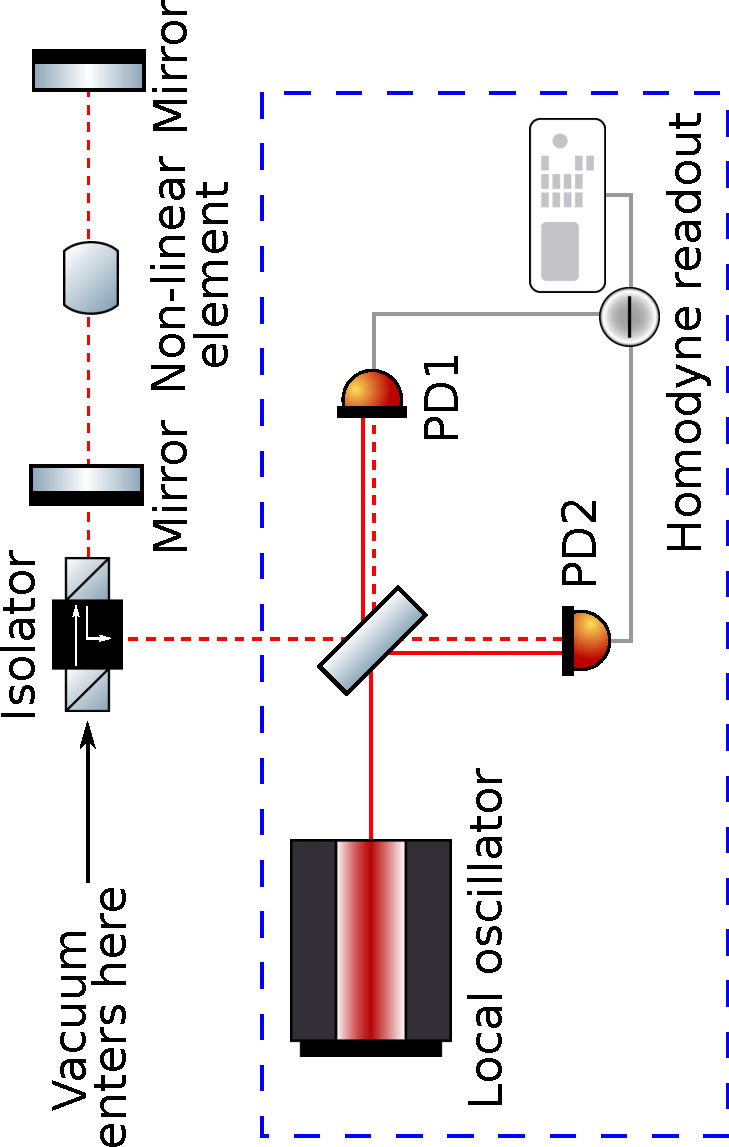
\includegraphics[width=0.45\textwidth]{figures/squeezed_cavity.pdf}
	\end{center}
	\caption{Configuration of squeezed cavity. A non-linear element is placed inside of a Fabry-Perot overcoupled cavity, an isolator lets vacuum fluctuations in and sends the squeezed states reflected from the cavity into a homodyne readout scheme. This configuration is used to test the \code{nle} component and build up to the aLIGO configuration shown in Fig.~\ref{fig:aLIGO_configuration}. In the derived analytics in Appendix~\ref{app:squeezed_cavity_analytics}, it is assumed that the only port for the vacuum fluctuations to enter is the input mirror to the cavity.}
	\label{fig:squeezed_cavity}
\end{figure}

\subsection{Analytics}

% approximate noise sources/vacuum to just come from ...
To first test the non-linear element we consider a simpler system than aLIGO, a squeezed cavity, as shown in Fig.~\ref{fig:squeezed_cavity}. This consists of a non-linear element inside of a cavity, and homodyne readout to detect the squeezed vacuum of quantum noise. An isolator is included to redirect the squeezed output. We assume that one of the mirrors is fully reflective (therefore the cavity is overcoupled) and that both mirrors are lossless. We assume that only port in the system for vacuum fluctuations to enter through is the input into the cavity. We also assume that the only other noise source in the system is the laser noise in the local oscillator (which will cancel out as usual in balanced homodyne readout).

% leave the actual derivation to an appendix
We derive the analytics for this system, getting an expression for the power spectral density (PSD) of the homodyne intensity, $S_{\mathrm{HomI}}(\Omega)$, in terms of the parameters of the cavity (the reflectivity of the input mirror, the length and tuning), the squeezer (gain and squeezer angle), and the local oscillator (amplitude and homodyne angle). We use Mathematica~\cite{mathematica} to simplify expressions. See Appendix~\ref{app:squeezed_cavity_analytics} for the full derivation and formulae.


\subsubsection{Threshold}
% threshold results, operating above threshold isn’t physically meaningful for the approximations made to reach these analytics

\begin{figure}[ht]
	\begin{center}
	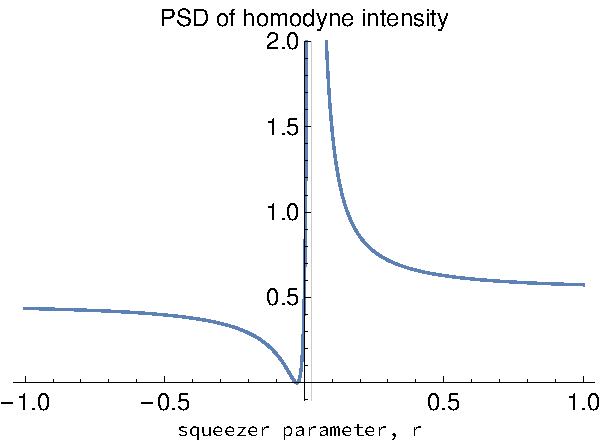
\includegraphics[width=0.45\textwidth]{figures/not_main_PSD_vs_r.pdf}
	\end{center}
	\caption{Homodyne intensity against squeezer parameter for a squeezed cavity. This figure shows the result from derived analytics for the absolute value of the PSD of homodyne intensity, normalised by the value with no squeezing. This figure shows a zero at $r = - 0.0263$ and a pole at $r = 0.0263$, known as the threshold. The behaviour above threshold is not of concern as some assumptions made in the analytics break down there and aLIGO operates well below threshold.}
	\label{fig:not_main_PSD_vs_r}
\end{figure}

\begin{figure*}
	\begin{center}
	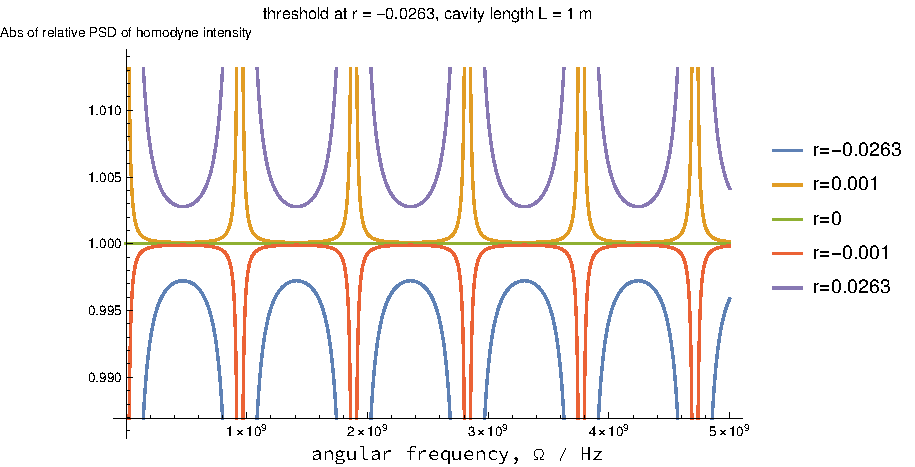
\includegraphics[width=0.7\textwidth]{figures/not_main_PSD_vs_freq.pdf}
	\end{center}
	\caption{Homodyne intensity against angular frequency offset around the carrier for a squeezed cavity. This figure shows a detail of the result from derived analytics for the absolute value of the PSD of homodyne intensity, normalised by the value with no squeezing, for various different squeezer parameters. This figure shows resonances with an FSR of $0.94248 \times 10^9$ Hz for the non-zero squeezer parameters. Off resonance, the difference between different squeezer parameters is far smaller, with the difference between positive and negative threshold being less than $1\%$.}
	\label{fig:not_main_PSD_vs_freq}
\end{figure*}

We first consider the behaviour at the carrier frequency of the absolute value of the (double-sided) PSD against the squeezer parameter, i.e.\ $\abs{S_{\mathrm{HomI}}(0)}$ against $r$ (alt.\ $r_\mathrm{sqz}$). We do this for a tuned, $1$ m long cavity, with the input mirror having reflectivity $r_1 = 0.9$, both squeezer and homodyne angle zero (squeezing and readout in the same quadrature), and amplitude $A = 1$ (in suitable units, see derivation), shown in Fig.~\ref{fig:not_main_PSD_vs_r}. This yields a pole at around $r_\mathrm{Thresh} = 0.0263$ (estimated numerically with Mathematica), known as the threshold value for the squeezer. The PSD also has a zero at $r = -r_\mathrm{Thresh}$ and limits to $0.5$ as $\abs{r}$ increases past threshold. Note that the squeezer parameter taking a negative value is equivalent to it taking the absolute value of that value and the squeezer angle changing by $\pi/2$, as in, switching to squeezing in the other quadrature.


The explanation for this behaviour lies in the assumptions made in the analytics. In particular, we assumed that the pump laser for the squeezer, which is its energy source, was essentially an undepletable reservoir. This meant that when we pumped in phase with the noise we could endlessly amplify and we when pumped out of phase we could completely cancel the noise, these two conditions exactly occur when threshold is reached. Physically this is not the case and pump depletion requires a Hamiltonian model of the system to analyse properly. This means that the analytics derived here break at threshold, similarly, any results above threshold are unphysical.
This could be an issue for modelling, except that the aLIGO squeezer operates normally well below threshold, where the model is reasonably accurate and so can be used to study aLIGO.


We are also interested in the behaviour at some frequency offset $\Omega$ relative to the behaviour at the carrier frequency, i.e.\ $\abs{S_{\mathrm{HomI}}(\Omega)/S_{\mathrm{HomI}}(0)}$ against $\Omega$. For the same parameters as above except for a selection of different squeezer parameters, this is shown in Fig.~\ref{fig:not_main_PSD_vs_freq}. For all non-zero squeezer parameters, it shows resonances every $9.42$ GHz (radians). At each resonance, the threshold values go to infinity and zero, while off resonance they are different from the carrier frequency but remain on the same scale (with difference of order $10^{-3}$).


\subsection{Testing the non-linear element in Finesse}

\begin{figure}[ht]
	\begin{center}
	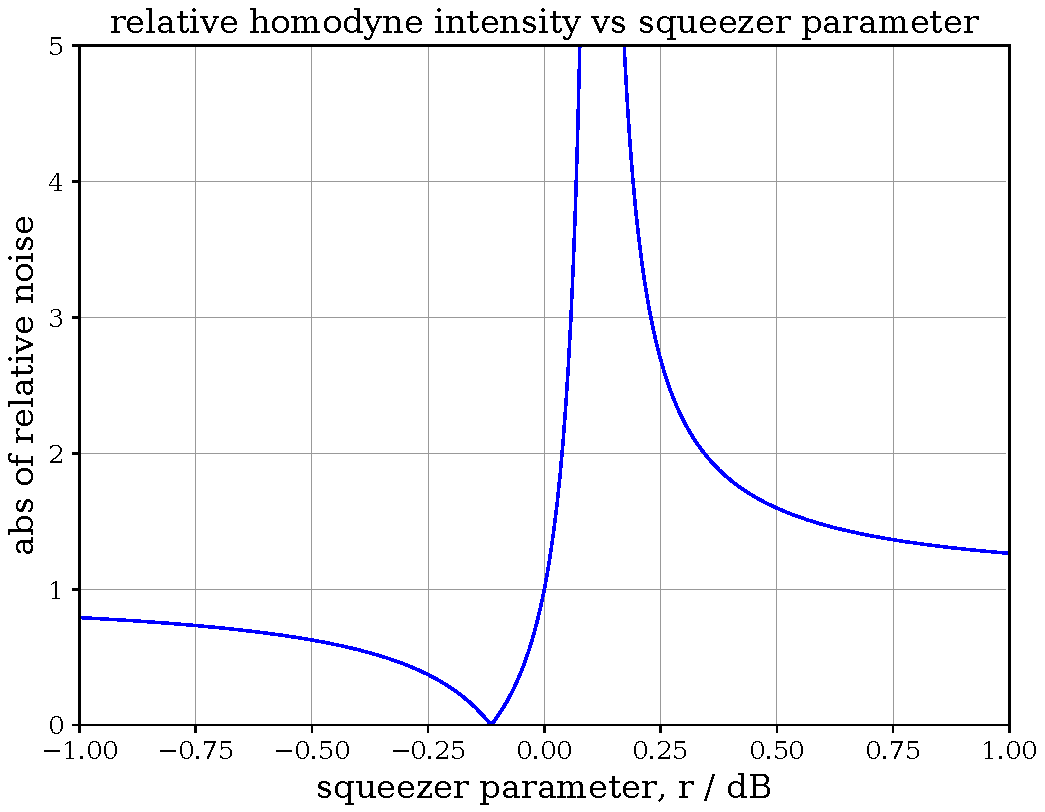
\includegraphics[width=0.45\textwidth]{figures/pykat_relative_qhd_vs_r.pdf}
	\end{center}
	\caption{Homodyne intensity against squeezer parameter for a squeezed cavity. This figure shows the result from a Finesse model for the absolute value of the \code{qhd} readout (which is the ASD of the homodyne intensity), normalised by the value with no squeezing. This figure shows similar behaviour to Fig.~\ref{fig:not_main_PSD_vs_r} with a threshold value of $r = 0.144$. If this threshold value is converted to dB, accounting for differing conventions, then the model and the analytics are found to agree, which is a good test of the \code{nle} component.}
	\label{fig:pykat_relative_qhd_vs_r}
\end{figure}

\begin{figure*}
	\begin{center}
	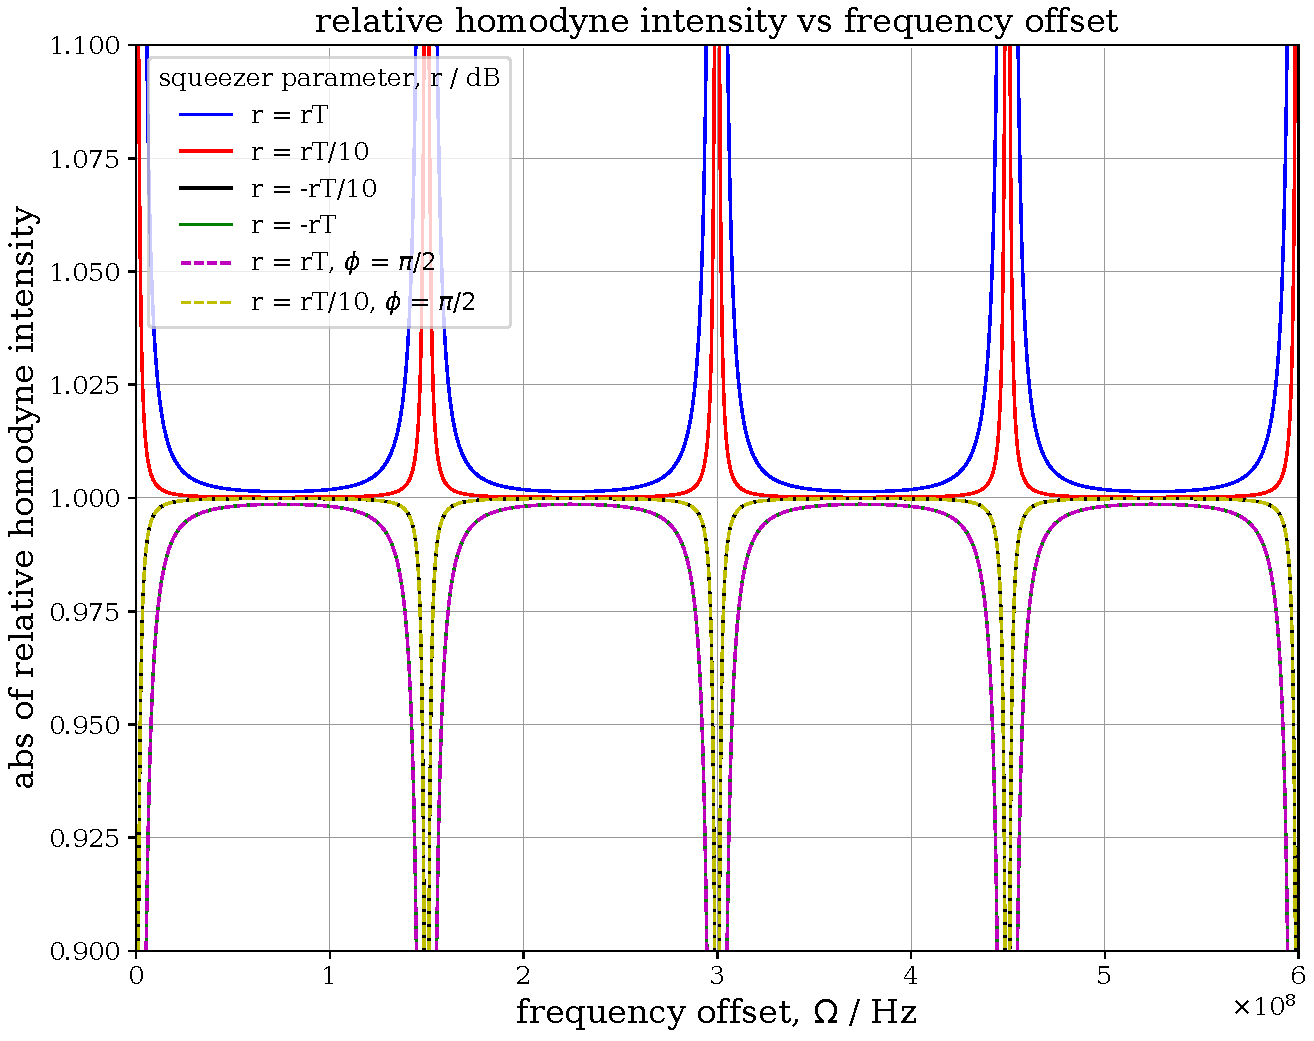
\includegraphics[width=0.7\textwidth]{figures/pykat_relative_qhd_vs_freq.pdf}
	\end{center}
	\caption{Homodyne intensity against angular frequency offset around the carrier for a squeezed cavity. This figure shows a detail of the result from a model in Finesse for the absolute value of the \code{qhd} readout (which is the ASD of the homodyne intensity), normalised by the value with no squeezing, for various different squeezer parameters (quote in terms of the threshold $r_T = 0.144$) and a couple of different squeezer angles. This figure shows resonances with an FSR of $0.94185 \times 10^9$ Hz for the non-zero squeezer parameters. The behaviour for the different squeezer parameters is similar to Fig.~\ref{fig:not_main_PSD_vs_freq}. This figures also demonstrates that a negative squeezer parameter is equivalent to the positive squeezer parameter but with $\pi/2$ squeezer angle, which is explained best with the ball and stick / noise ellipse in Section~\ref{sec:squeezing} and that changing the squeezer angle by $\pi/2$ means that the other quadrature is now being squeezed.}
	\label{fig:pykat_relative_qhd_vs_freq}
\end{figure*}

We model the squeezed cavity in Finesse with the \code{nle} component as the squeezer and \code{qhd} for homodyne readout of the quantum noise. We do this for the same parameters as above and only consider the relative spectral density to avoid worrying about units of amplitude. Note that \code{qhd} calculates amplitude spectral density rather than PSD, which under a logarithm gives a factor of two between them, further confusing the definitions of dB.


% rThresh and \Omega values are the same, convert to dB and check angular freq
The behaviour of the relative homodyne intensity against the squeezer parameter is shown in Fig.~\ref{fig:pykat_relative_qhd_vs_r}. The shape of the response is similar to the analytics. The squeezer parameter axis shows the input to \code{nle} which is in ``dB'' calculated as $r_{\mathrm{nle}} = 10 \log_{10}(e^{r_\mathrm{sqz}})$. Python quotes the threshold value as $0.144$ (here shown to three s.f.) which agrees with the analytics, $0.114 \approx 10 \log_{10}(e^{0.0263})$, with negligible uncertainty.


% FSR is 1.5 since L = 1
The behaviour against the frequency offset is shown in Fig.~\ref{fig:pykat_relative_qhd_vs_freq}. Again, the response is similar in shape to the analytics.
The angular FSR ($2 \pi \mathrm{FSR}$) for the model is (up to numerical error) $0.94185 \times 10^9$ Hz.
The angular FSR in the analytics is $0.94248 \times 10^9$ Hz.
The theoretical value for $L = 1$ m is $2 \pi \mathrm{FSR} = 2 \pi c/(2 L) \approx 0.94183 \times 10^9$ Hz.
Therefore, the error between the model and the analytics is on the order of $10^5$ Hz and the error between the model and the theoretical value is on the order of $10^3$ Hz.
The behaviour of the model against frequency for different squeezer parameters is also similar to the analytics.


Overall, the \code{nle} component successfully models the squeezed cavity, with the consideration for the particular definition of dB used. Now, having passed the first test, we want to test the implementation in a gravitational wave detector to then start predicting the behaviour of proposed designs.


\section{Modelling advanced gravitational wave detector configurations}
\label{sec:aLIGOcomparison}

\subsection{Analytics for the reduced aLIGO configuration}

% get source from Vaishali
We use analytics for the coupled cavity system (shown in Fig.~\ref{fig:aLIGO_as_coupled_cavities}) derived in Refs.~\cite{Korobko_2019,SOMIYA2016521}. Recall that this system is an approximation, albeit a good one, of the simplified aLIGO configuration (shown in Fig.~\ref{fig:aLIGO_configuration}). In addition, the input/output relation and the calculation of the coupled cavity pole are both only approximate. We claim below that these approximations are responsible for the rest of the discrepancy between the analytics and the Finesse model, after first correcting for the implementation in Finesse.


\subsection{Finesse model of aLIGO}

% table of aLIGO parameters used in Finesse model and analytics
\begin{table}[ht]
	\centering
	\begin{tabular}{l|ll}
	 & analytics & Finesse \\ \hline
	Arm length / m & 3994.5 & 3994.5 \\
	SRC length / m & 319 & 319 \\
	Power on beamsplitter / kW & 5.35 & 5.35 \\
	Power in arms / kW & 758.9 & 758.9 \\
	SRM power transmission & 0.12 & 0.12 \\
	ITM power transmission & 0.014 & 0.014 \\
	\textit{Gain input to internal squeezer} & 0.06 & $5 \log_{10}(e^{0.06})$ \\
	Maximum sensitivity / $1/\sqrt{\mathrm{Hz}}$ & $3.95 \times 10^{-25}$ & $4.16 \times 10^{-25}$ \\
	Peak frequency / kHz & 2.49 & 2.51
	\end{tabular}%
	\caption{Parameters and results of aLIGO. This table compares the input parameters and resultant peak quantum noise limited sensitivity of the existing analytics for the reduced aLIGO configuration shown in Fig.~\ref{fig:aLIGO_as_coupled_cavities} and a model in Finesse of the simplified aLIGO configuration shown in Fig.~\ref{fig:aLIGO_configuration}. To achieve peak sensitivity within $5\%$ fractional error, note that the input to the internal squeezer is converted to dB as $5 \log_{10}$ which includes a correction factor of four.}
	\label{tab:aLIGO_parameters}
\end{table}

\begin{figure*}[ht]
	\begin{center}
	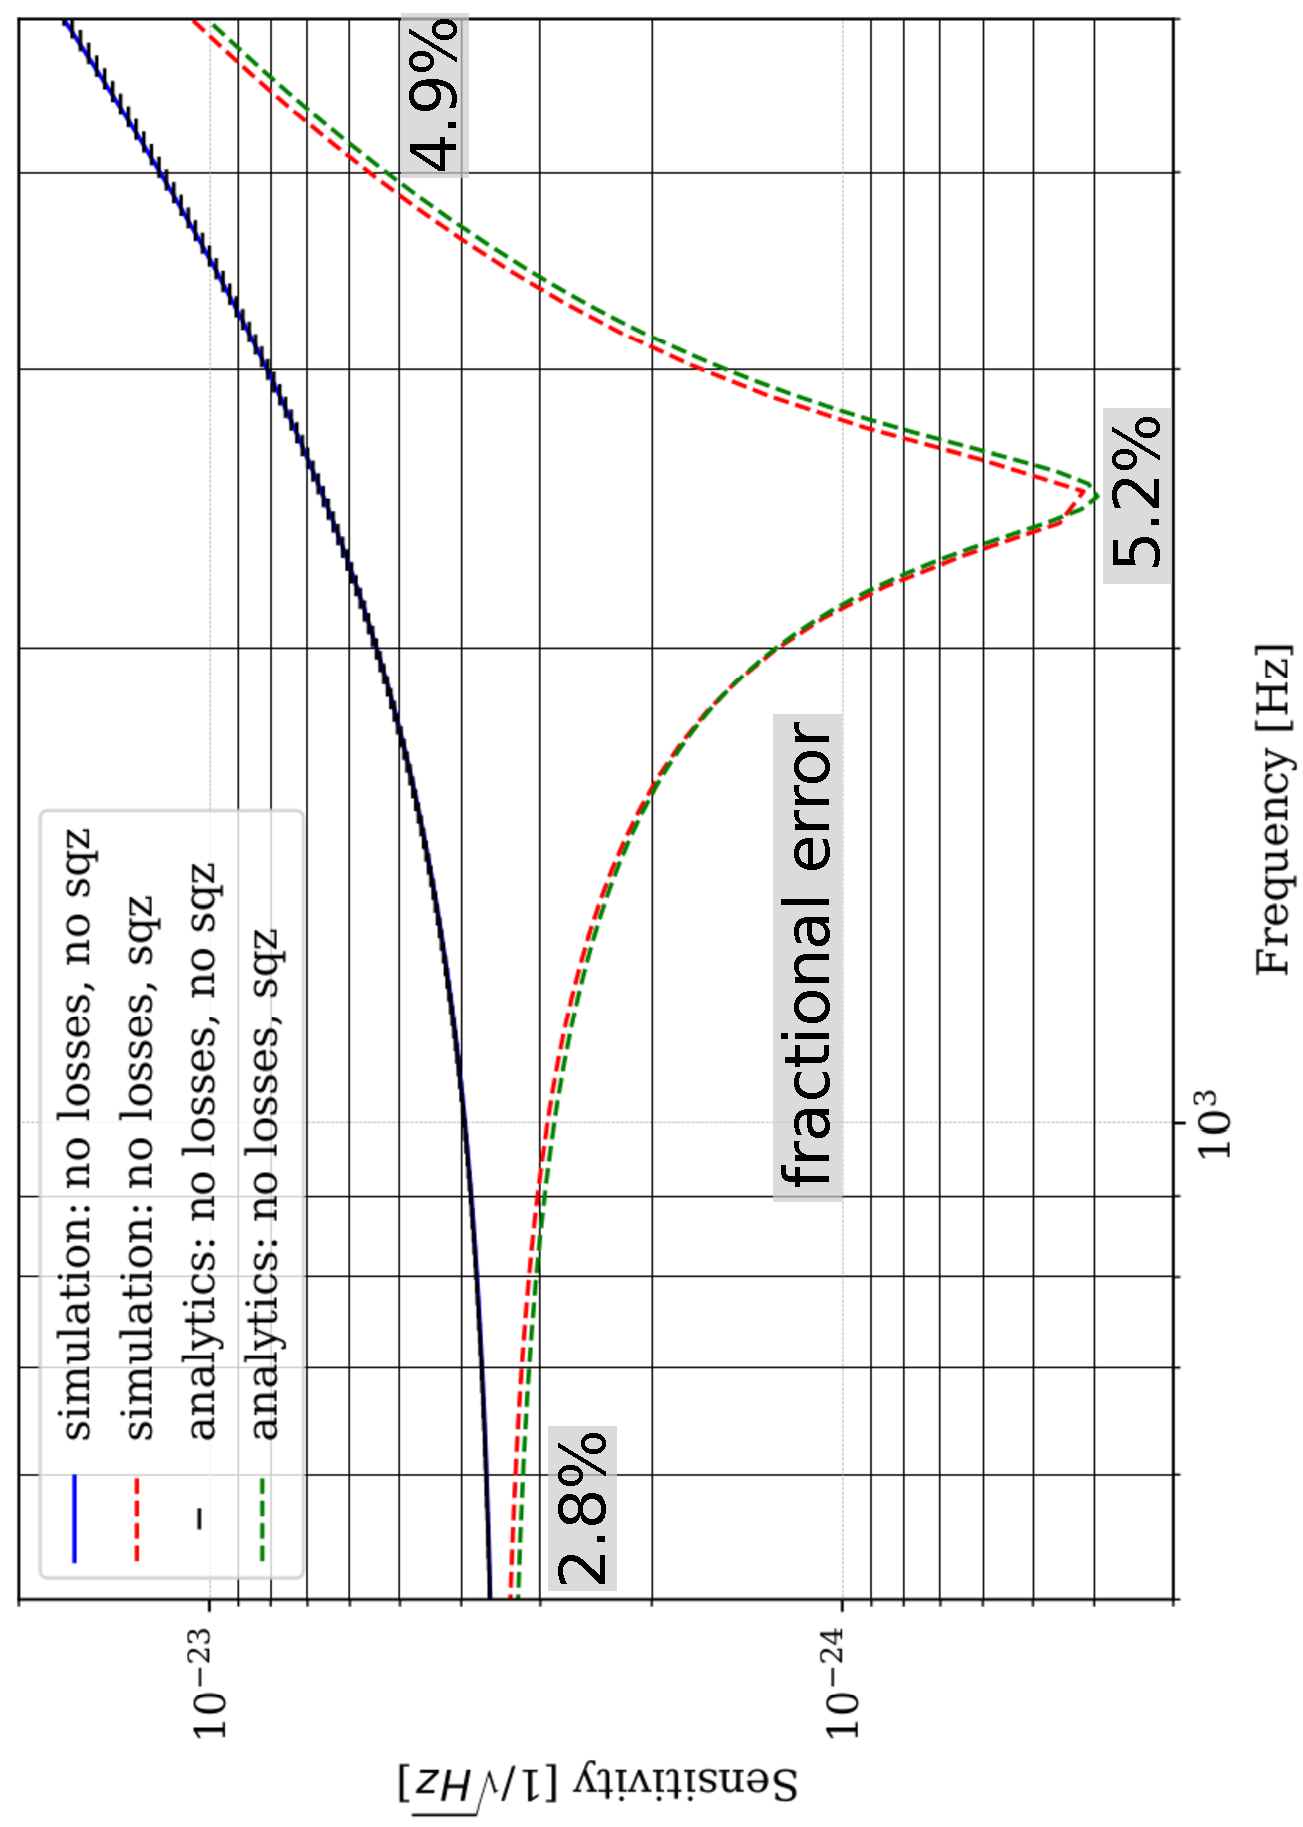
\includegraphics[height=0.65\textwidth, angle=-90]{figures/sqz_aLIGO_analytics_v_simulation_with_fractional_errors.pdf}
	\end{center}
	\caption{Quantum noise limited strain sensitivity of aLIGO for a long SRC (319 m) with internal squeezing. This figure compares the results from existing analytics against a Finesse model, with and without internal squeezing. Without squeezing the two agree. With squeezing, the model has a fractional error of approximately $5\%$ to the analytics, this figure shows the fractional error sampled at three points: the start and end of the plotting window and at the peak. The peak sensitivity with squeezing in the analytics is $3.95 \times 10^{-25}\, 1/\sqrt{\mathrm{Hz}}$ and in the model is $4.16 \times 10^{-25} \, 1/\sqrt{\mathrm{Hz}}$.}
	\label{fig:sqz_aLIGO_analytics_v_simulation}
\end{figure*}

We model the simplified, lossless aLIGO configuration (shown in Fig.~\ref{fig:aLIGO_configuration}) in Finesse with internal squeezing using the \code{nle} component. We study a long SRC configuration here, although the agreement between the analytics and Finesse is similar for different parameters. Internal squeezing configurations with lengths of the SRC of 53 m and 2 km generate the signal and noise transfer functions and sensitivity shown in Fig.~\ref{fig:src_transfer_functions}. A summary of some of the parameters used here is shown in Table~\ref{tab:aLIGO_parameters}. Note that the squeezer in the analytics takes the $r_\mathrm{sqz} = 0.06$ parameter as input while the \code{nle} takes the gain in dB (defined as $10 \log_{10}(e^\mathrm{sqz})$ against convention) as input. Due to another factor of two, however, here we input only $5 \log_{10}(e^\mathrm{sqz})$ into the Finesse model, explained below.


It is worth briefly explaining how we made sure that the Finesse model was simulating the same system as the reduced configuration in the analytics, i.e.\ how we got the parameters in Table~\ref{tab:aLIGO_parameters} to agree. Firstly, we checked that the model was acting as an interferometer, at one stage the beamsplitter was oriented incorrectly. Then, we tuned the interferometer as to have the operating point at the dark fringe, i.e.\ made sure no power from the main laser was at the output of the beamsplitter. Finally, we matched the power in the arms between the model and the analytics by removing all losses, matching the mirror transmitivities, and setting the same power on the beamsplitter by making the power recycling mirror transparent and setting the input laser power to match.


% comparison for long SRC with internal squeezing
A comparison of sensitivity of the analytics and Finesse is shown in Fig.~\ref{fig:sqz_aLIGO_analytics_v_simulation}. With the squeezer turned off, the agreement is nearly exact (to numerical error). With the squeezer turned on, the sensitivity is similar between the analytics and the Finesse model, with an average fractional error of $5\%$ calculated as $$\mathrm{fractional\; error} = \frac{\mathrm{model} - \mathrm{analytics}}{\mathrm{analytics}}.$$
This remaining error we attribute to the approximations made in the analytics, in particular the calculation of the coupled cavity pole, and therefore suspect that the Finesse model is more accurate, although we are not certain. Even if the error is in the Finesse model, it is small enough for the predictions made using the model to still be useful in determining the optimal detector configuration.


\subsubsection{Explaining the discrepancy in dB}

% different def of dB gives a factor of 2
To recap, the squeezer in the analytics takes $r_\mathrm{sqz}$ as input and produces a gain in dB calculated as $20 \log_{10}(e^\mathrm{sqz})$. In Finesse, the \code{nle} components takes a gain value as input but calculates dB as only $10 \log_{10}(e^\mathrm{sqz})$, therefore producing twice the amount of squeezing than expected, as shown in Fig.~\ref{fig:testing_Finesse_squeezers}. This means that given the $r_\mathrm{sqz} = 0.06$ input into the analytics, we need to halve the gain to account for the difference in definitions in dB, and input into \code{nle} $10 \log_{10}(e^\mathrm{sqz})$.


% double passing of NLE gives another factor of 2
As seen in Fig.~\ref{fig:sqz_aLIGO_analytics_v_simulation}, however, the correct value to pass to \code{nle} is $5 \log_{10}(e^\mathrm{sqz})$, so where is the second factor of two? As mentioned in Section~\ref{sec:squeezing}, physical squeezer crystals are directional, meaning that they will only squeeze states incident from one side (and travelling in the direction of the pump laser), letting those incident from the other through unchanged. The implementation of \code{nle} is, however, direction-less, meaning that it squeezes from both sides. When placed in a cavity it produces twice the amount of squeezing than expected. Therefore, given a squeezer parameter (not in dB), the gain in dB to pass to \code{nle} is half as small due to different definitions of dB and half as small again due to the direction-less-ness of the component. This second factor of two was not evident in the squeezed cavity results because there the squeezer in the analytics was directionless.


% Is the recommendation to Daniel Brown to both fix the dB and perhaps make nle a directional component (will squeeze light from n1 to n2, but will just let light through n2 to n1)?
Overall, the \code{nle} component successfully models the simplified aLIGO configuration up some error likely due to approximations in the analytics, with the caveat that the gain input must be corrected to account for the nature of the implementation. This is a good result and resolves, positively, the testing of the \code{nle} component that we set out to do. For the sake of consistency, we recommend that the \code{nle} component be modified to calculate the gain as $20 \log_{10}(e^\mathrm{sqz})$ and possibly made directional.


\subsection{Optimisation}

\begin{figure*}[ht]
	\begin{center}
	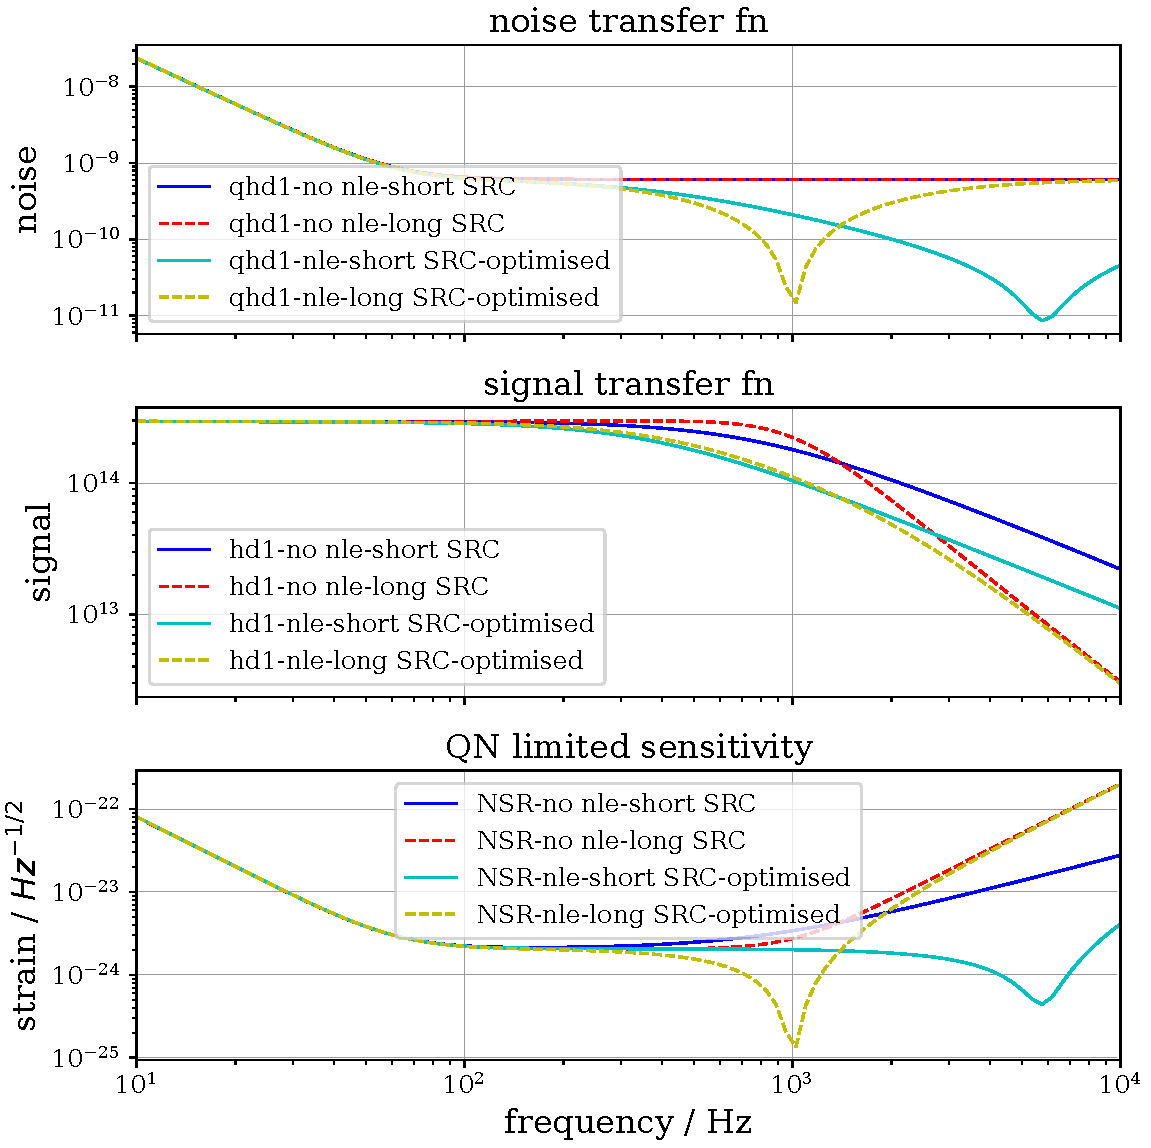
\includegraphics[width=0.6\textwidth]{figures/aLIGO_optimum_sensitivity_comparison.pdf}
	\end{center}
	\caption{The quantum noise (top panel), signal transfer function (middle panel), and quantum noise limited strain sensitivity (bottom panel) for aLIGO. This figure shows the results from a model in Finesse optimised to achieve the best sensitivity between 900 Hz and 3 kHz by varying the squeezer parameters and homodyne angle, for two fixed lengths of the SRC (53 m and 2 km).
	See Figure~\ref{fig:src_transfer_functions} for an explanation of the layout and trends shown. This figure shows almost an order of magnitude improvement in peak sensitivity above the results in Figure~\ref{fig:src_transfer_functions}. For configurations with too many physical effects to describe analytically, this optimisation seems very useful for detector design.}
	\label{fig:aLIGO_optimum_sensitivity_comparison}
\end{figure*}

% reason to use python is to optimise
Having successfully shown that Finesse can model the aLIGO configuration, we can now use PyKat to optimise the sensitivity in some band against whatever parameters we like. Here we only do this briefly, as a demonstration of the ability, but more broadly this is a key benefit of Finesse.


We optimise the quantum noise limited sensitivity within a high frequency band of 900 Hz to 3 kHz for fixed lengths of SRC of 53 m and 2 km, the results are shown in Fig.~\ref{fig:aLIGO_optimum_sensitivity_comparison}. This band is easily changed and was chosen to represent a detector tuned to a source in the low kHz region. The optimisation was allowed to vary the squeezer gain, the squeezer angle, and the homodyne angle. Once again the results show the high peak and short bandwidth of the long SRC which achieves a sensitivity of $1.36 \times 10^{-25}\; 1/\sqrt{\mathrm{Hz}}$. It achieves this at a non-zero squeezer angle of $0.014^\circ$, which is surprising and not yet understood (although it could just be the optimisation routine). Allowing the optimisation to vary additionally the length of the SRC, the power transmission of the SRM, and the tuning of the SRM led to the optimisation getting stuck near the various initial values given, for reasons not yet understood.


%%%%%%%%%%%%%%%%%%%%%%%%%%%%%%%%%%%%%%%%%%
\section{Future work}
\label{sec:future_work}

We’ve shown that Finesse can successfully model internal squeezing and have then used it to demonstrate the benefits of a long SRC. Here we detail other proposed configurations and how Finesse could be used to evaluate their efficacy.


% optimisation
Fixing the many parameter optimisation would improve Finesse’s usefulness in designing the configuration to achieve the best sensitivity in the desired band. Potential fixes to getting stuck in local minima would be to test many different initial conditions in some efficient way or constrain the problem more in some way. Alternatively, the current cost function (which is “maximise quantum noise SNR in a given band”) could be replaced by some other choice in the literature, such as Eq.~1 in Ref.~\cite{Miao_2014} or Eq.~8 in Ref.~\cite{Martynov_2019}, which may be less prone to local minima and/or more physically useful to detector design.


% losses
We’ve ignored losses to simplify these initial tests, however, losses should be included in any realistic model. The complication with introducing a loss is that it then acts as a port for vacuum fluctuations, the coupling of which needs to then be included in the analytics. Finesse handles this complication itself and so introducing realistic losses into the model would be easy, albeit more difficult to write the analytics for.


% other noise sources
Similarly, we’ve focussed on quantum noise here because it limits the high frequency sensitivity of current detectors. A more realistic model would include other sorts of noise sources along with control systems. Finesse is able to handle control signals and so they could be added in. Finesse can handle other noise sources, up to the limitations of the model in how the noise can affect the components.
% Either the modelling would need to ignore those noise sources or some cleverness with injecting suitable sidebands would be required.


% detuned long SRC, non-degenerate squeezing
As for different proposed configurations, two changes would be detuning the long SRC and non-degenerate squeezing. Detuning should allow for more control of the bandwidth of the detector and so allow for more sources to be seen.
Detuning the long SRC is something we started to investigate by allowing the optimisation routine to change the tuning of the SRM, investigating this further would amount to fixing the optimisation as above.
Non-degenerate squeezing is when the produced entangled photons from the squeezer, the signal and the idler, are at different frequencies and so see the interferometer differently. This would require the addition of a new component to Finesse able to be internal to the configuration, similar to \code{nle}, but is otherwise achievable to model. The motivation for internal non-degenerate squeezing is to be able to replace (potentially) a ``white-light cavity'' (not explained here, but see Ref.~\cite{white-light-resonators}) and get the same broadband improvement without the complications of the stability, the high mechanical quality factor, and the low required thermal noise of the ``white-light cavity''.


% other limitations of finesse in its current form that can be overcome?


\section{Conclusions}
\label{sec:conclusions}
% can be quite short!

% remotivate
In this report, we use Finesse to model advanced gravitational wave detector configurations proposed to improve on those in use. These detectors are complex and the analytics are tedious to derive for each proposed configuration. Finesse, and optical modelling more generally, allows for quick results and determination of the efficacy of a configuration.


% sqz cavity, derived analytics
We were interested in improving the high frequency (kHz) sensitivity of the detectors in order to see new sources, like the late states of binary neutron star--neutron star mergers. Since the current detectors are limited by quantum noise at high frequencies, we investigated configurations involving internal squeezing in a long SRC that were proposed to reduce shot noise at high frequencies without affecting the low frequency sensitivity of the detector. In order to do internal squeezing in Finesse, we first needed to test the \code{nle} component. We started by considering a simpler system of a squeezed cavity and used derived analytics to test the component in Finesse. The component successfully recovered the threshold (and FSR) values for the squeezed cavity.


% aLIGO, recommendation
We then considered a simplified configuration of aLIGO, and used existing analytics to test the component in Finesse. This was successful up to a $5\%$ fractional error attributed to approximations made in the analytics, with the caveat that the input to the component had to be corrected for different conventions of dB and the directionality of the squeezer.
For the sake of consistency, we recommend that the \code{nle} component be changed to match convention.


% optimisation
Work in optimising the high frequency quantum noise limited sensitivity by varying the squeezer and SRC parameters is ongoing, but has already demonstrated how Finesse can be used to find optimum detector configurations. All this and more future work, such as modelling  exotic configurations, is now possible since we can trust the component that has passed all of our tests.


\begin{acknowledgments}
The authors wish to thank the developers of Finesse for their great, open software.
The authors also wish to thank the OzGrav-ANU squeezer group for their continued advice and support.

\end{acknowledgments}


%%%%%%%%%%%%%%%%%%%%%%%%%%%%%%%%%%%%%%%%%%
\appendix
\section{Squeezed cavity analytics}
\label{app:squeezed_cavity_analytics}

We want the PSD of the homodyne intensity, $S_{\mathrm{HomI}}(\Omega)$, for the squeezed cavity. We proceed in four steps:
\begin{itemize}
\item finding the transfer matrix for the empty cavity
\item borrowing the solution to arrive at the quadratures at the photodiodes
\item computing the Fourier spectrum of the time averaged intensity
\item using properties of the quantum noise quadratures from Ref.~\cite{Danilishin_2012} to arrive at the result
\end{itemize}

\subsection{Derivation}

\subsubsection{Transfer matrix for a cavity}

% fix position of this figure later
\begin{figure}[ht]
	\begin{center}
	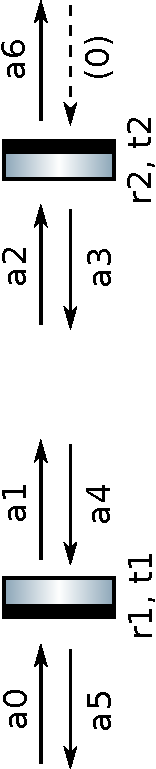
\includegraphics[width=0.45\textwidth]{figures/empty_cavity_amplitudes.pdf}
	\end{center}
	\caption{Labelled electric field amplitudes for empty cavity, used in deriving matrix solution for the reflected field $a_5$ in terms of the incident field $a_0$.}
	\label{fig:empty_cavity_amplitudes}
\end{figure}

Consider an empty two-mirror cavity with reflectivities $r_1, r_2$ and transmitivities $t_1, t_2$. For simplicity we assume mirror 1 is lossless and mirror two is perfectly reflective $r_2 = 1, t_2 = 0$. Light $a_0(\Omega)$ is incident on mirror 1, where $a_0$ is a vector of the two quadratures in the frequency domain (see Section~\ref{sec:squeezing}). Let $a_j$ for $j = 1, \ldots, 6$ be similar and defined as in Fig.~\ref{fig:empty_cavity_amplitudes}. We use the mirror phase convention of no change on transmission and reflection from one of the sides and $\pi$ on reflection from the other side. The transmission and reflection matrices are therefore $R_i = r_i I,\; T_i = t_i I$, where $i = 1, 2$ and $I$ is the $2 \times 2$ identity matrix. Let the propagation matrix from one mirror to the other be $P$ which we construct later. Therefore, the amplitudes are related by
\begin{align*}
a_1 &= T_1 a_0 + R_1 a_4\\
a_2 &= P a_1\\
a_3 &= R_2 a_2 \\
a_4 &= P a_3\\
a_5 &= T_1 a_4 - R_1 a_0\\
a_6 &= T_2 a_2
\end{align*}
Solving the set of equations
\begin{align*}
a_4 &= P R_2 P (T_1 a_0 + R_1 a_4) \\
a_4 &= (I - P R_2 P R_1)^{-1} P R_2 P T_1 a_0 \\
a_5 &= \left(T_1 (I - P R_2 P R_1)^{-1} P R_2 P T_1 - R_1\right) a_0
\end{align*}
We get an expression for the reflected field off the cavity, $a_5$.


The propagation matrix $P$ across free space depends on the length and tuning of the space. Let the cavity be $D = L + \delta l$ long. Then the propagation across free space is
\begin{align*}
P(L, \delta l) &= \exp\left(i\frac{\Omega (L + \delta l)}{c}\right) \;\mathrm{Rot}\left(\frac{\omega_0 \delta l}{c}\right) \\
\mathrm{Rot}(\phi) &= \begin{bmatrix}
\cos(\phi) & -\sin(\phi)\\ 
\sin(\phi) & \cos(\phi)
\end{bmatrix}
\end{align*}
We assume that $\Omega \ll \omega_0$ and so $\frac{\Omega \delta l}{c} \ll 1$. Let the angular tuning be $\psi = \frac{\omega_0 \delta l}{c}$. Therefore $$P(L, \delta l) = \exp\left(i\frac{\Omega L}{c}\right) \;\mathrm{Rot}\left(\psi\right)$$

\subsubsection{Quadratures at the photodiodes}

To incorporate the squeezer we borrow the above solution but change the propagation matrix to
\begin{align*}
	\begin{gathered}
	\tilde{P}(L, \delta l, r, \phi) = P\left(\frac{L}{2}, \frac{\delta l}{2}\right) \mathrm{Sqz}(r, \phi) P\left(\frac{L}{2}, \frac{\delta l}{2}\right) \\
	\mathrm{Sqz}(r, \phi) =\\
	\begin{bmatrix}
	\cos(2 \phi) \sinh(r) + \cosh(r) & \sin(2\phi) \sinh(r)\\ 
	\sin(2\phi) \sinh(r) & -\cos(2 \phi) \sinh(r) + \cosh(r)
	\end{bmatrix}
	\end{gathered}
\end{align*}
Where $r = r_\mathrm{sqz}$ is the squeezer parameter (not in dB) and $\phi$ is the squeezer angle. Note that this means that the light gets squeezed from both directions by the squeezer. This is not what physically happens but is how \code{nle} is implemented, so for ease of comparison we choose this convention. Note that this is different to the directional squeezer in the analytics in Section~\ref{sec:aLIGOcomparison}.


Referring to Fig.~\ref{fig:squeezed_cavity}, let $n = a_0$ be the vacuum incident on the cavity, $a$ be the laser noise, and let the local oscillator itself be
$$A = A_0 \begin{bmatrix}
\cos(\theta)\\ 
\sin(\theta)
\end{bmatrix}$$
For homodyne angle $\theta$ and amplitude $A_0$. The field reflected off the cavity is
$$n_r = \left(t_1 (I - r_1 \tilde{P}^2)^{-1} \tilde{P}^2 t_1 - r_1 \right) n$$


For a 50/50 beamsplitter and negligible propagation lengths outside the cavity the fields (as quadrature vectors, frequency dependent) at the two photodiodes are therefore
\begin{align*}
b_1 &= \frac{1}{\sqrt{2}} \left( n_r + A + a\right) \\
b_2 &= \frac{1}{\sqrt{2}} \left( n_r - A - a\right)
\end{align*}

\subsubsection{Fourier spectrum of the time averaged intensity}

Consider the time average of the intensity at photodiode 1. Need to take inverse Fourier transform of frequency domain field, let tilde denote time domain. Note that depending on quadrature convention there may need to be a constant squared out the front of the intensity to fix the units, we later drop this constant anyway so I won’t write it. 
\begin{align*}
\tilde{b}_1 &= \begin{bmatrix}
\tilde{b}_{1,c}\\ 
\tilde{b}_{1,s}
\end{bmatrix} \\
\expect{\tilde{I}_1(t)} &= \expect{\abs{\tilde{b}_{1,c} \cos(\omega_0 t) + \tilde{b}_{1,s} \sin(\omega_0 t)}^2}
\end{align*}
Assuming that the time domain quadrature are Hermitian allows the absolute value squared to be expanded. Also assume that the quadratures are slowly changing with respect to $\omega_0$. Taking time averages we note $\expect{\cos(\omega_0 t) \sin(\omega_0 t)} = 0$ and $\expect{\cos^2} = \expect{\sin^2} = 1/2$. This leaves
$$\expect{\tilde{I}_1} = \frac{1}{2} \left( \tilde{b}_{1,c}^2 + \tilde{b}_{1,s}^2 \right)$$


Splitting the quadratures into a constant $B$ and a time varying part $\tilde{b}'$ with average zero and assuming that the time varying part is small with respect to the constant (this is true for the noise compared to the local oscillator). We expand the quadratures squared and drop the time varying part squared terms.
$$\expect{\tilde{I}_1} = \frac{1}{2} \left( B_{1,c}^2 + B_{1,s}^2 + 2 \left( B_{1,c} \tilde{b}_{1,c}' + B_{1,s} \tilde{b}_{1,s}' \right) \right)$$


Now taking Fourier transform to return to frequency domain, and dropping the (DC) constant term since we are only interested in the quantum noise. Recall that tildes indicated time domain, so we just drop them.
$$\expect{I_1} = B_{1,c} b_{1,c}' + B_{1,s} b_{1,s}'$$


We claim that these $B$ and $b'$ are the constant and frequency dependant parts of the original quadrature $b$. This amounts to $B$ being the local oscillator, e.g.\ $B_{1,c} = 1/\sqrt{2} A_0 \cos(\theta)$, and $b'$ being the noise terms in $b$, i.e.\ $1/\sqrt{2} (n_r \pm a)$. The homodyne intensity, $\mathrm{HomI}$, is then
$$\mathrm{HomI} = \expect{I_1 - I_2} = B_{1,c} b_{1,c}' + B_{1,s} b_{1,s}' - B_{2,c} b_{2,c}' - B_{2,s} b_{2,s}'$$


Substituting the quadratures at the photodiodes and simplifying reveals that the homodyne intensity doesn’t depend on $a$, the laser noise of the local oscillator, as expected. Let $n_c$ and $n_s$ be the quadratures of the original vacuum input $n$.
$$\mathrm{HomI} = \frac{A_0(g_1 n_c + g_2 n_s)}{g_3}$$

\begingroup
\allowdisplaybreaks
\begin{align*}
g_1 &= -\cosh ^2(r) e^{\frac{2 i L \Omega }{c}} (\cos (\theta ) \left(2 r_1^2+t_1^2\right) \cos (2 \psi )\\
	&+t_1^2	\sin (\theta ) \sin (2 \psi )) \\
	&-\cos (\theta ) \sinh ^2(r) \left(2 r_1^2+t_1^2\right) e^{\frac{2 i L \Omega
	}{c}}\\
	&-t_1^2 \cos (\theta ) \sinh (2 r) \cos (\psi ) \cos (2 \phi ) e^{\frac{2 i L \Omega }{c}}\\
	&-t_1^2 \sin (\theta )
	\sinh (2 r) \cos (\psi ) \sin (2 \phi ) e^{\frac{2 i L \Omega }{c}}\\
	&+r_1^3 \cos (\theta ) e^{\frac{4 i L \Omega
	}{c}}+r_1 t_1^2 \cos (\theta ) e^{\frac{4 i L \Omega }{c}}+r_1 \cos (\theta ) \\
g_2 &= \cosh ^2(r) e^{\frac{2 i L \Omega }{c}} (t_1^2 \cos (\theta ) \sin (2 \psi )\\
	&-\sin (\theta ) \left(2 r_1^2+t_1^2\right) \cos (2 \psi ))\\
	&+\sin (\theta ) \left(-\sinh ^2(r) (2 r_1^2+t_1^2\right)
	e^{\frac{2 i L \Omega }{c}}\\
	&+t_1^2 \sinh (2 r) \cos (\psi ) \cos (2 \phi ) e^{\frac{2 i L \Omega }{c}}\\
	&+r_1^3	e^{\frac{4 i L \Omega }{c}}+r_1 t_1^2 e^{\frac{4 i L \Omega }{c}}+r_1)\\
	&-4 t_1^2 \cos (\theta ) \sinh (r) \cosh (r) \cos (\psi ) \sin (\phi ) \cos (\phi ) e^{\frac{2 i L \Omega }{c}} \\
g_3 &= 1 + r_1^2 e^{\frac{4 i L \Omega}{c}} - 2 e^{\frac{2 i L \Omega}{c}} \sinh(r)^2 \\
	&- 2 e^{\frac{2 i L \Omega}{c}} r_1 \cos(2 \psi) \cosh(r)^2 
\end{align*}
\endgroup

\subsubsection{PSD of the homodyne intensity}

Recall the definition of PSD from Section~\ref{sec:squeezing}, and noting that $S, \mathrm{HomI}, n$ should all have hats (\,$\hat{}$\,) but we drop them to reduce clutter.
$$S_\mathrm{HomI}(\Omega) 2 \pi \delta(\Omega - \Omega') = \langle0| \mathrm{HomI}(\Omega) \circ \mathrm{HomI}^\dagger(\Omega') |0\rangle$$

Assuming that the homodyne intensity is hermitian, and expanding out the symmetric products we get
\begin{align*}
S_\mathrm{HomI}(\Omega) 2 \pi \delta(\Omega - \Omega') &= \frac{A_0^2}{g_3(\Omega) g_3(\Omega')} \\
&\cdot \langle0| g_1(\Omega) g_1(\Omega') (n_c(\Omega) \circ n_c(\Omega'))\\
&+ g_2(\Omega) g_2(\Omega') (n_s(\Omega) \circ n_s(\Omega')) \\
&+ g_1(\Omega) g_2(\Omega') (n_c(\Omega) \circ n_s(\Omega')) \\
&+ g_2(\Omega) g_1(\Omega') (n_s(\Omega) \circ n_c(\Omega')) |0\rangle
\end{align*}


From pg.~38 of Ref.~\cite{Danilishin_2012}, for the quantum noise we have the following relations (the factor of $1/2$ is from the choice of using a double-sided PSD).
\begin{align*}
\langle0|n_c(\Omega) \circ n_c(\Omega')|0\rangle &= \frac{1}{2} 2 \pi \delta(\Omega - \Omega') \\
\langle0|n_s(\Omega) \circ n_s(\Omega')|0\rangle &= \frac{1}{2} 2 \pi \delta(\Omega - \Omega') \\
\langle0|n_c(\Omega) \circ n_s(\Omega')|0\rangle &= 0
\end{align*}

Substituting these relations in we arrive at the result, the PSD of the homodyne intensity. For plotting purposes we set $A_0 = 1$.
$$S_\mathrm{HomI}(\Omega) = \frac{A_0^2 \left( g_1(\Omega)^2 + g_2(\Omega)^2 \right)}{g_3(\Omega)^2}$$


%%%%%%%%%%%%%%%%%%%%%%%%%%%%%%%%%%%%%%%%%%
\nocite{*}
\bibliographystyle{myunsrt}
\bibliography{bib}


\end{document}
